\documentclass[]{article}
\usepackage{lmodern}
\usepackage{amssymb,amsmath}
\usepackage{ifxetex,ifluatex}
\usepackage{fixltx2e} % provides \textsubscript
\ifnum 0\ifxetex 1\fi\ifluatex 1\fi=0 % if pdftex
  \usepackage[T1]{fontenc}
  \usepackage[utf8]{inputenc}
\else % if luatex or xelatex
  \ifxetex
    \usepackage{mathspec}
  \else
    \usepackage{fontspec}
  \fi
  \defaultfontfeatures{Ligatures=TeX,Scale=MatchLowercase}
\fi
% use upquote if available, for straight quotes in verbatim environments
\IfFileExists{upquote.sty}{\usepackage{upquote}}{}
% use microtype if available
\IfFileExists{microtype.sty}{%
\usepackage{microtype}
\UseMicrotypeSet[protrusion]{basicmath} % disable protrusion for tt fonts
}{}
\usepackage[margin=1in]{geometry}
\usepackage{hyperref}
\hypersetup{unicode=true,
            pdftitle={Tennis},
            pdfauthor={Michael Roberts, Min Liu, Nicholas Hovens, Zhexu Zhang},
            pdfborder={0 0 0},
            breaklinks=true}
\urlstyle{same}  % don't use monospace font for urls
\usepackage{color}
\usepackage{fancyvrb}
\newcommand{\VerbBar}{|}
\newcommand{\VERB}{\Verb[commandchars=\\\{\}]}
\DefineVerbatimEnvironment{Highlighting}{Verbatim}{commandchars=\\\{\}}
% Add ',fontsize=\small' for more characters per line
\usepackage{framed}
\definecolor{shadecolor}{RGB}{248,248,248}
\newenvironment{Shaded}{\begin{snugshade}}{\end{snugshade}}
\newcommand{\KeywordTok}[1]{\textcolor[rgb]{0.13,0.29,0.53}{\textbf{#1}}}
\newcommand{\DataTypeTok}[1]{\textcolor[rgb]{0.13,0.29,0.53}{#1}}
\newcommand{\DecValTok}[1]{\textcolor[rgb]{0.00,0.00,0.81}{#1}}
\newcommand{\BaseNTok}[1]{\textcolor[rgb]{0.00,0.00,0.81}{#1}}
\newcommand{\FloatTok}[1]{\textcolor[rgb]{0.00,0.00,0.81}{#1}}
\newcommand{\ConstantTok}[1]{\textcolor[rgb]{0.00,0.00,0.00}{#1}}
\newcommand{\CharTok}[1]{\textcolor[rgb]{0.31,0.60,0.02}{#1}}
\newcommand{\SpecialCharTok}[1]{\textcolor[rgb]{0.00,0.00,0.00}{#1}}
\newcommand{\StringTok}[1]{\textcolor[rgb]{0.31,0.60,0.02}{#1}}
\newcommand{\VerbatimStringTok}[1]{\textcolor[rgb]{0.31,0.60,0.02}{#1}}
\newcommand{\SpecialStringTok}[1]{\textcolor[rgb]{0.31,0.60,0.02}{#1}}
\newcommand{\ImportTok}[1]{#1}
\newcommand{\CommentTok}[1]{\textcolor[rgb]{0.56,0.35,0.01}{\textit{#1}}}
\newcommand{\DocumentationTok}[1]{\textcolor[rgb]{0.56,0.35,0.01}{\textbf{\textit{#1}}}}
\newcommand{\AnnotationTok}[1]{\textcolor[rgb]{0.56,0.35,0.01}{\textbf{\textit{#1}}}}
\newcommand{\CommentVarTok}[1]{\textcolor[rgb]{0.56,0.35,0.01}{\textbf{\textit{#1}}}}
\newcommand{\OtherTok}[1]{\textcolor[rgb]{0.56,0.35,0.01}{#1}}
\newcommand{\FunctionTok}[1]{\textcolor[rgb]{0.00,0.00,0.00}{#1}}
\newcommand{\VariableTok}[1]{\textcolor[rgb]{0.00,0.00,0.00}{#1}}
\newcommand{\ControlFlowTok}[1]{\textcolor[rgb]{0.13,0.29,0.53}{\textbf{#1}}}
\newcommand{\OperatorTok}[1]{\textcolor[rgb]{0.81,0.36,0.00}{\textbf{#1}}}
\newcommand{\BuiltInTok}[1]{#1}
\newcommand{\ExtensionTok}[1]{#1}
\newcommand{\PreprocessorTok}[1]{\textcolor[rgb]{0.56,0.35,0.01}{\textit{#1}}}
\newcommand{\AttributeTok}[1]{\textcolor[rgb]{0.77,0.63,0.00}{#1}}
\newcommand{\RegionMarkerTok}[1]{#1}
\newcommand{\InformationTok}[1]{\textcolor[rgb]{0.56,0.35,0.01}{\textbf{\textit{#1}}}}
\newcommand{\WarningTok}[1]{\textcolor[rgb]{0.56,0.35,0.01}{\textbf{\textit{#1}}}}
\newcommand{\AlertTok}[1]{\textcolor[rgb]{0.94,0.16,0.16}{#1}}
\newcommand{\ErrorTok}[1]{\textcolor[rgb]{0.64,0.00,0.00}{\textbf{#1}}}
\newcommand{\NormalTok}[1]{#1}
\usepackage{graphicx,grffile}
\makeatletter
\def\maxwidth{\ifdim\Gin@nat@width>\linewidth\linewidth\else\Gin@nat@width\fi}
\def\maxheight{\ifdim\Gin@nat@height>\textheight\textheight\else\Gin@nat@height\fi}
\makeatother
% Scale images if necessary, so that they will not overflow the page
% margins by default, and it is still possible to overwrite the defaults
% using explicit options in \includegraphics[width, height, ...]{}
\setkeys{Gin}{width=\maxwidth,height=\maxheight,keepaspectratio}
\IfFileExists{parskip.sty}{%
\usepackage{parskip}
}{% else
\setlength{\parindent}{0pt}
\setlength{\parskip}{6pt plus 2pt minus 1pt}
}
\setlength{\emergencystretch}{3em}  % prevent overfull lines
\providecommand{\tightlist}{%
  \setlength{\itemsep}{0pt}\setlength{\parskip}{0pt}}
\setcounter{secnumdepth}{0}
% Redefines (sub)paragraphs to behave more like sections
\ifx\paragraph\undefined\else
\let\oldparagraph\paragraph
\renewcommand{\paragraph}[1]{\oldparagraph{#1}\mbox{}}
\fi
\ifx\subparagraph\undefined\else
\let\oldsubparagraph\subparagraph
\renewcommand{\subparagraph}[1]{\oldsubparagraph{#1}\mbox{}}
\fi

%%% Use protect on footnotes to avoid problems with footnotes in titles
\let\rmarkdownfootnote\footnote%
\def\footnote{\protect\rmarkdownfootnote}

%%% Change title format to be more compact
\usepackage{titling}

% Create subtitle command for use in maketitle
\providecommand{\subtitle}[1]{
  \posttitle{
    \begin{center}\large#1\end{center}
    }
}

\setlength{\droptitle}{-2em}

  \title{Tennis}
    \pretitle{\vspace{\droptitle}\centering\huge}
  \posttitle{\par}
    \author{Michael Roberts, Min Liu, Nicholas Hovens, Zhexu Zhang}
    \preauthor{\centering\large\emph}
  \postauthor{\par}
      \predate{\centering\large\emph}
  \postdate{\par}
    \date{6 May 2019}


\begin{document}
\maketitle

\subsection{Introduction}\label{introduction}

\textbf{Team members:} Michael Roberts, Min Liu, Nicholas Hovens, Zhexu
Zhang

\subsubsection{What is tennis}\label{what-is-tennis}

via GIPHY

\begin{itemize}
\tightlist
\item
  tennis is a racket sport
\item
  can be played individually against a single opponent or between two
  teams of two players each
\item
  each player uses the racket to hit the tennis ball over the net to
  their opponents side of the court
\item
  the object of the game is to hit the ball in such a way that the
  opponent cannot play a valid return
\item
  the player who plays the winning shot gets a point
\end{itemize}

\subsubsection{About our data}\label{about-our-data}

\begin{itemize}
\tightlist
\item
  we used the ``deuce'' package to obtain our data
  \url{https://github.com/skoval/deuce}
\end{itemize}

\subsection{Australian Men's ATP
Rankings}\label{australian-mens-atp-rankings}

\begin{itemize}
\tightlist
\item
  The ATP rankings are used by the Association of Tennis Professionals
  (ATP) to determine qualification for entry as well as the seeding of
  players in all singles and doubles tournaments
\item
  The rankings are updated every Monday, so I have used the first Monday
  of every year from 2001 - 2018 for the following analysis
\item
  I will be focusing on the singles rankings
\end{itemize}

\subsubsection{Cleaning of the data}\label{cleaning-of-the-data}

\begin{Shaded}
\begin{Highlighting}[]
\NormalTok{atp_players1 <-}\StringTok{ }\NormalTok{atp_players }\OperatorTok
\StringTok{ }\KeywordTok{select}\NormalTok{(name, player_id, country_code)}\OperatorTok
\StringTok{ }\KeywordTok{filter}\NormalTok{(country_code }\OperatorTok{==}\StringTok{ "AUS"}\NormalTok{)}

\NormalTok{atp_rankings1 <-}\StringTok{ }\NormalTok{atp_rankings }\OperatorTok
\StringTok{ }\KeywordTok{select}\NormalTok{(ranking, player_id, date)}\OperatorTok
\StringTok{ }\KeywordTok{filter}\NormalTok{(ranking }\OperatorTok{<=}\StringTok{ }\DecValTok{100}\NormalTok{) }

\NormalTok{atp_data <-}\StringTok{ }\NormalTok{atp_players1 }\OperatorTok
\StringTok{  }\KeywordTok{left_join}\NormalTok{(atp_rankings1, }\DataTypeTok{by =} \StringTok{"player_id"}\NormalTok{) }\OperatorTok
\StringTok{  }\KeywordTok{mutate}\NormalTok{(}\DataTypeTok{year =} \KeywordTok{year}\NormalTok{(date), }
         \DataTypeTok{day =} \KeywordTok{day}\NormalTok{(date),}
         \DataTypeTok{month =} \KeywordTok{month}\NormalTok{(date, }\DataTypeTok{label=}\OtherTok{TRUE}\NormalTok{, }\DataTypeTok{abbr=}\OtherTok{TRUE}\NormalTok{))}\CommentTok{#, locale = "English"))}

\NormalTok{current_atprankings <-}\StringTok{ }\KeywordTok{fetch_atp_rankings}\NormalTok{(}\StringTok{"2019-05-20"}\NormalTok{, }\DataTypeTok{min_rank =} \DecValTok{1}\NormalTok{, }\DataTypeTok{max_rank =} \DecValTok{100}\NormalTok{) }\OperatorTok
\StringTok{ }\KeywordTok{select}\NormalTok{(player, rank, date) }\OperatorTok
\StringTok{  }\KeywordTok{rename}\NormalTok{(}\KeywordTok{c}\NormalTok{(}\StringTok{"player"}\NormalTok{ =}\StringTok{ "name"}\NormalTok{, }\StringTok{"rank"}\NormalTok{ =}\StringTok{ "ranking"}\NormalTok{))}

\NormalTok{currentatp_data <-}\StringTok{ }\NormalTok{atp_players1 }\OperatorTok
\StringTok{  }\KeywordTok{full_join}\NormalTok{(current_atprankings, }\DataTypeTok{by =} \StringTok{"name"}\NormalTok{) }\OperatorTok
\StringTok{  }\KeywordTok{na.omit}\NormalTok{(currentatp_data)}
\end{Highlighting}
\end{Shaded}

\begin{itemize}
\tightlist
\item
  the atp\_players data was read in, relevant variables were selected
  and the country was filtered to display only Australian players
\item
  the atp\_rankings data was read in, the relevant variables were
  selected and the rankings were filtered to show the top 100
\item
  the atp players and atp rankings data was then combined via a left
  join so that the rankings can be attributed to name
\item
  the date of the rankings was also split into 3 variables: year, month
  and day
\item
  the same was done for the current ATP rankings (fetch\_atp\_rankings),
  a couple of the variables were renamed so they could be joined to the
  atp\_players data and the NA values were omitted
\end{itemize}

\subsubsection{Individual Australian players ATP
rankings}\label{individual-australian-players-atp-rankings}

\begin{center}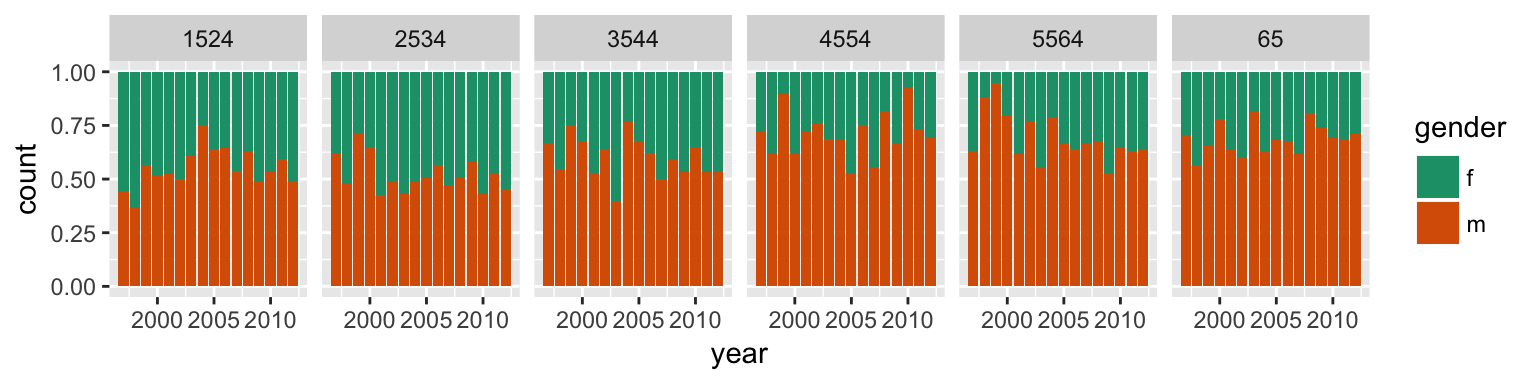
\includegraphics{Submitted_Group_Project_Storyboard_files/figure-latex/unnamed-chunk-2-1} \end{center}

\begin{itemize}
\tightlist
\item
  Lleyton Hewitt has been our highest ranked (1) male tennis player
  since 2001
\item
  He was ranked in the top 100 from 2001 - 2012, then 2013 - 2015
\end{itemize}

via GIPHY

\begin{itemize}
\tightlist
\item
  We have had at least 1 player ranked in the top 100 each year since
  2001
\item
  We have had at least 1 player ranked in the top 50 each year except
  2009 and 2011
\item
  Australia hasn't had any men ranked in the top 10 since 2006
\end{itemize}

\subsubsection{Total Australian's in the ATP top 100 per
year}\label{total-australians-in-the-atp-top-100-per-year}

\begin{center}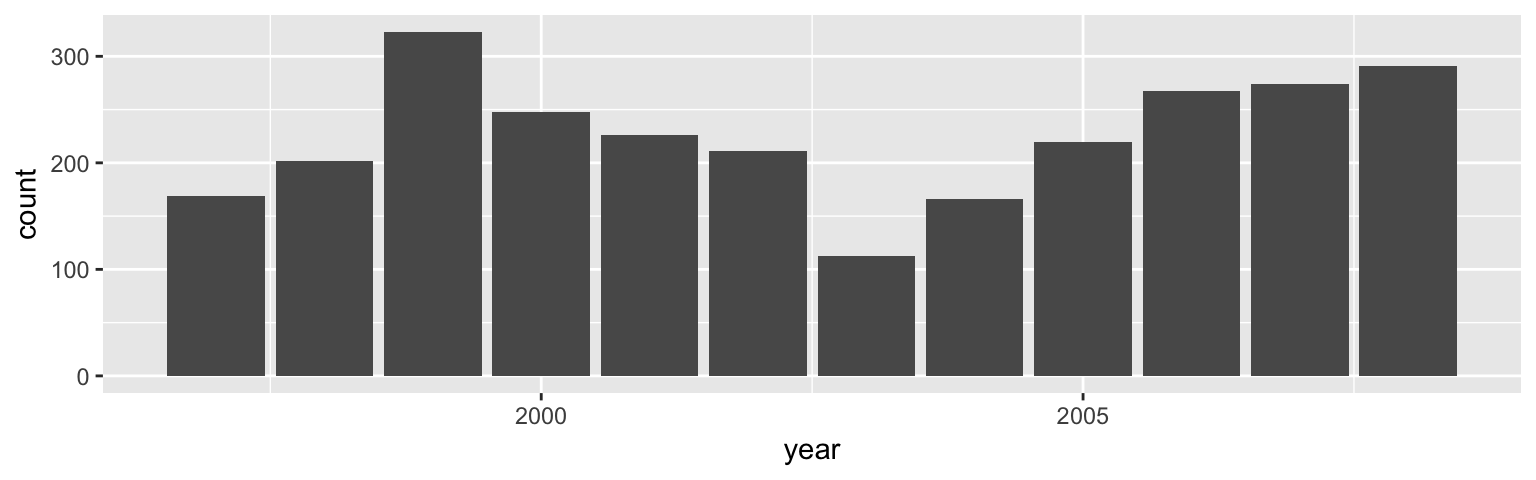
\includegraphics{Submitted_Group_Project_Storyboard_files/figure-latex/unnamed-chunk-3-1} \end{center}

\begin{itemize}
\tightlist
\item
  Between 2001-2018, 2001 saw the most Australian male tennis players in
  the top 100 with 7
\item
  Rapid decline after that with Australia seeing between 1 or 2 male
  tennis players in the top 100 from 2003 - 2012
\item
  Looks to be a steady increase from 2013 onwards
\end{itemize}

\subsubsection{Current Australian's in the top 100 ATP
Rankings}\label{current-australians-in-the-top-100-atp-rankings}

\begin{center}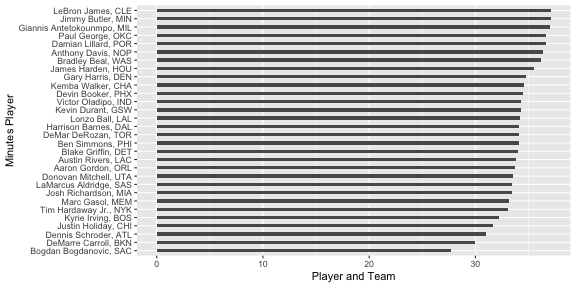
\includegraphics{Submitted_Group_Project_Storyboard_files/figure-latex/unnamed-chunk-4-1} \end{center}

\begin{itemize}
\tightlist
\item
  As of right now, Australia has 5 players ranked in the ATP top 100
\item
  Continues with the trending increase of Australian players in the ATP
  top 100
\item
  Highest Australian right now is Nick Kyrgios who is ranked at 36
\end{itemize}

via GIPHY

\subsubsection{Top ten countries with players in the ATP top 100 since
2001}\label{top-ten-countries-with-players-in-the-atp-top-100-since-2001}

\begin{center}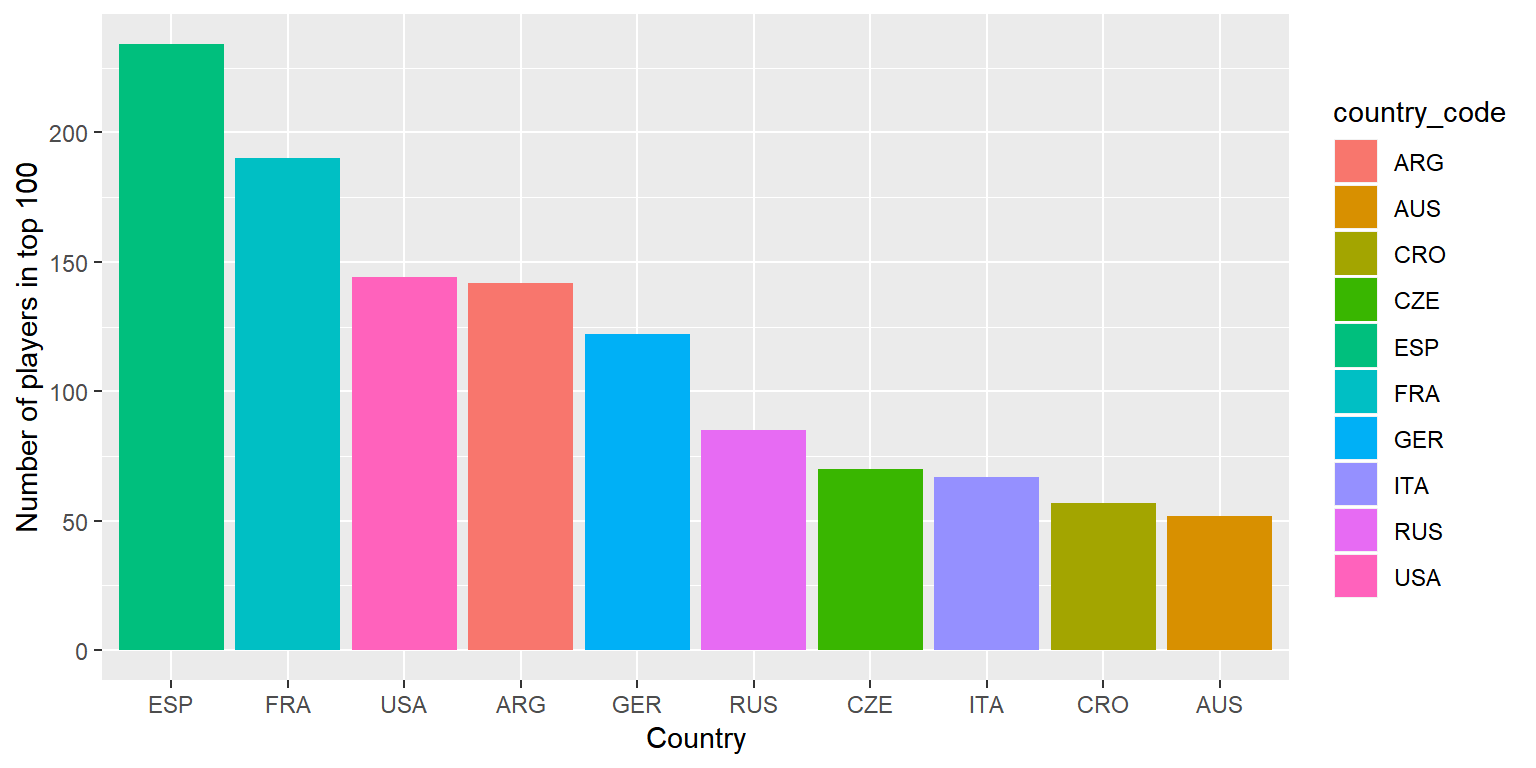
\includegraphics{Submitted_Group_Project_Storyboard_files/figure-latex/unnamed-chunk-5-1} \end{center}

\begin{itemize}
\tightlist
\item
  Spain has had the most players ranked in the top 100 since 2001 with
  234 players
\item
  Australia has had the 10th most with 52 players
\item
  7 of the countries in the top ten are from Europe
\end{itemize}

\subsection{Australian Women's WTA
Rankings}\label{australian-womens-wta-rankings}

\begin{itemize}
\tightlist
\item
  The WTA rankings are used by the Women's Tennis Association (WTA) to
  determine qualification for entry as well as the seeding of players in
  all singles and doubles tournaments
\item
  The rankings are updated every Monday, so I have used the first Monday
  of every year from 2001 - 2018 for the following analysis
\item
  I will be focusing on the singles rankings
\end{itemize}

\subsubsection{Cleaning of the data}\label{cleaning-of-the-data-1}

\begin{Shaded}
\begin{Highlighting}[]
\NormalTok{wta_players1 <-}\StringTok{ }\NormalTok{wta_players }\OperatorTok
\StringTok{ }\KeywordTok{select}\NormalTok{(name, player_id, country_code)}\OperatorTok
\StringTok{ }\KeywordTok{filter}\NormalTok{(country_code }\OperatorTok{==}\StringTok{ "AUS"}\NormalTok{)}

\NormalTok{wta_rankings1 <-}\StringTok{ }\NormalTok{wta_rankings }\OperatorTok
\StringTok{ }\KeywordTok{select}\NormalTok{(ranking, player_id, date)}\OperatorTok
\StringTok{ }\KeywordTok{filter}\NormalTok{(ranking }\OperatorTok{<=}\StringTok{ }\DecValTok{100}\NormalTok{) }

\NormalTok{wta_data <-}\StringTok{ }\NormalTok{wta_players1 }\OperatorTok
\StringTok{  }\KeywordTok{left_join}\NormalTok{(wta_rankings1, }\DataTypeTok{by =} \StringTok{"player_id"}\NormalTok{) }\OperatorTok
\StringTok{  }\KeywordTok{mutate}\NormalTok{(}\DataTypeTok{year =} \KeywordTok{year}\NormalTok{(date), }
         \DataTypeTok{day =} \KeywordTok{day}\NormalTok{(date),}
         \DataTypeTok{month =} \KeywordTok{month}\NormalTok{(date, }\DataTypeTok{label=}\OtherTok{TRUE}\NormalTok{, }\DataTypeTok{abbr=}\OtherTok{TRUE}\NormalTok{))}\CommentTok{#, locale = "English"))}

\NormalTok{wta_ausrankings <-}\StringTok{ }\NormalTok{wta_data }\OperatorTok
\StringTok{  }\KeywordTok{select}\NormalTok{(name, ranking, year, day, month) }\OperatorTok
\StringTok{  }\KeywordTok{filter}\NormalTok{(year }\OperatorTok{>}\StringTok{ }\DecValTok{2000}\NormalTok{, month }\OperatorTok{==}\StringTok{ "Jan"}\NormalTok{, day }\OperatorTok{<}\StringTok{ }\DecValTok{8}\NormalTok{)}

\NormalTok{current_wtarankings <-}\StringTok{ }\KeywordTok{fetch_wta_rankings}\NormalTok{(}\DataTypeTok{min_rank =} \DecValTok{1}\NormalTok{, }\DataTypeTok{max_rank =} \DecValTok{100}\NormalTok{) }\OperatorTok
\StringTok{  }\KeywordTok{select}\NormalTok{(player, nation, rank, date) }\OperatorTok
\StringTok{  }\KeywordTok{filter}\NormalTok{(nation }\OperatorTok{==}\StringTok{ "Australia"}\NormalTok{) }\OperatorTok
\end{Highlighting}
\end{Shaded}

\begin{itemize}
\tightlist
\item
  similar to the cleaning for the ATP rankings
\item
  wta\_players, wta\_rankings, fetch\_wta\_rankings were used to obtain
  the data
\end{itemize}

\subsubsection{Individual Australian players WTA
rankings}\label{individual-australian-players-wta-rankings}

\begin{center}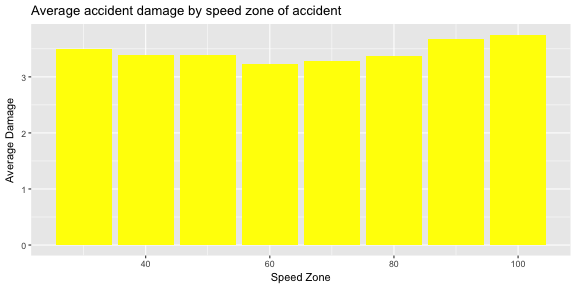
\includegraphics{Submitted_Group_Project_Storyboard_files/figure-latex/unnamed-chunk-7-1} \end{center}

\begin{itemize}
\tightlist
\item
  Samantha Stosur has been our highest ranked female tennis player (6)
  since 2001
\item
  She has been in the top 100 since 2005 and the top 25 from 2010 - 2015
\end{itemize}

via GIPHY

\begin{itemize}
\tightlist
\item
  Since 2001, there hasn't been a year with no Australian female tennis
  players in the top 100
\item
  Australia has had at least one female tennis player ranked in the top
  50 every year since 2001, except for 2009
\end{itemize}

\subsubsection{Total Australian's in the WTA top 100 per
year}\label{total-australians-in-the-wta-top-100-per-year}

\begin{center}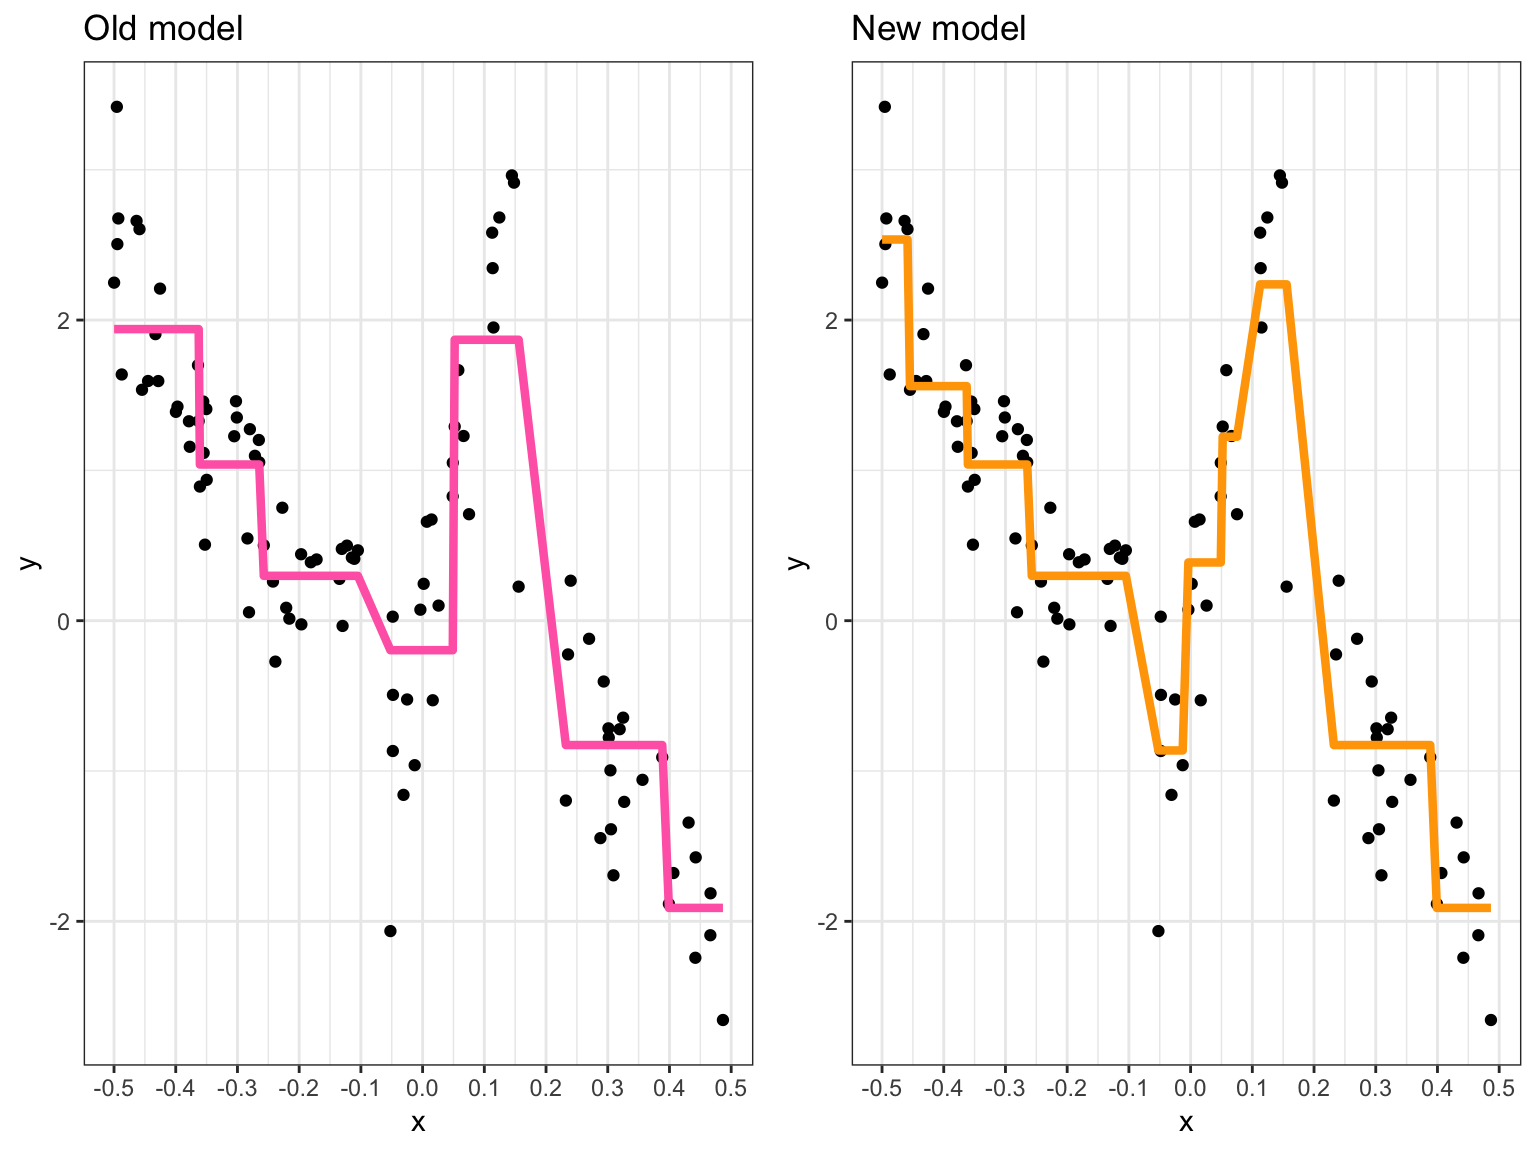
\includegraphics{Submitted_Group_Project_Storyboard_files/figure-latex/unnamed-chunk-8-1} \end{center}

\begin{itemize}
\tightlist
\item
  2002 and 2008 had the most female players in the top 100 with ten
\item
  2014 and 2017 had the least with two
\item
  Seems to be a steady decrease in players in the wta top 100 since 2008
\end{itemize}

\subsubsection{Current Australian's in the top 100 WTA
Rankings}\label{current-australians-in-the-top-100-wta-rankings}

\begin{center}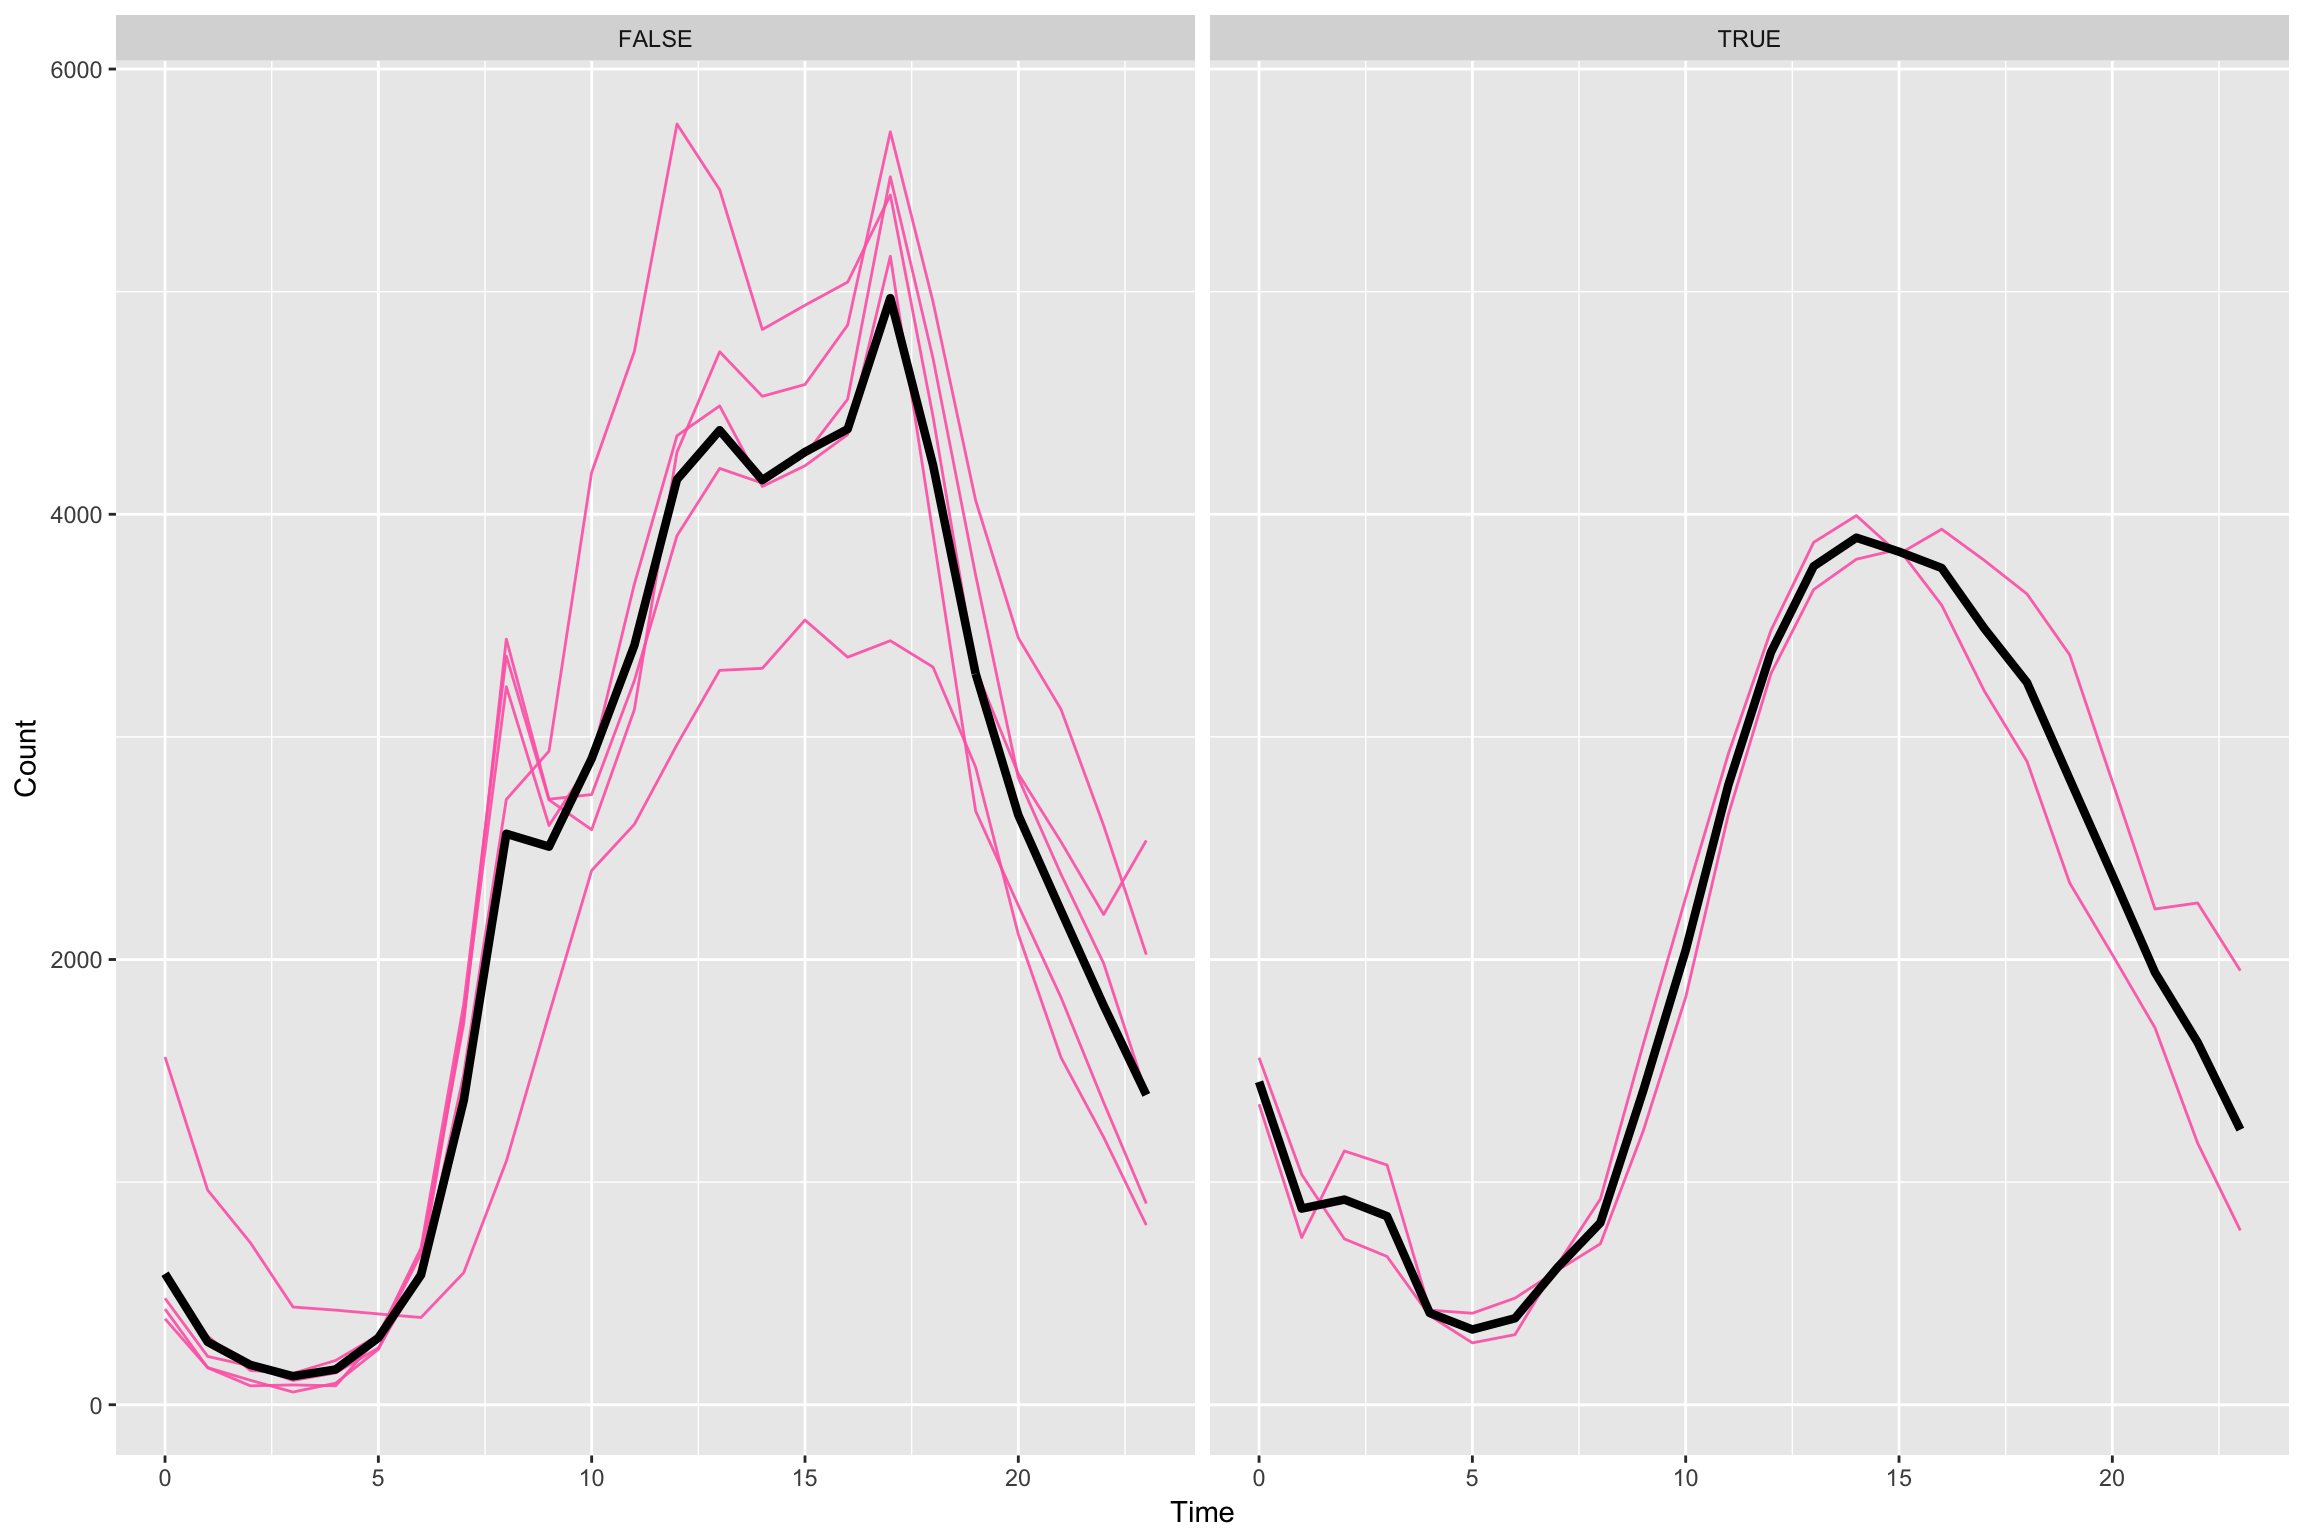
\includegraphics{Submitted_Group_Project_Storyboard_files/figure-latex/unnamed-chunk-9-1} \end{center}

\begin{itemize}
\tightlist
\item
  As of right now, Australia has 5 players ranked in the WTA top 100
\item
  This is the most Australia has had in the WTA top 100 since 2012
\item
  This could show the beginning of another rise in Australians in the
  WTA top 100
\item
  Highest Australian right now is Ash Barty who is ranked 8th
\end{itemize}

via GIPHY

\subsubsection{Top ten countries with players in the WTA top 100 since
2001}\label{top-ten-countries-with-players-in-the-wta-top-100-since-2001}

\begin{center}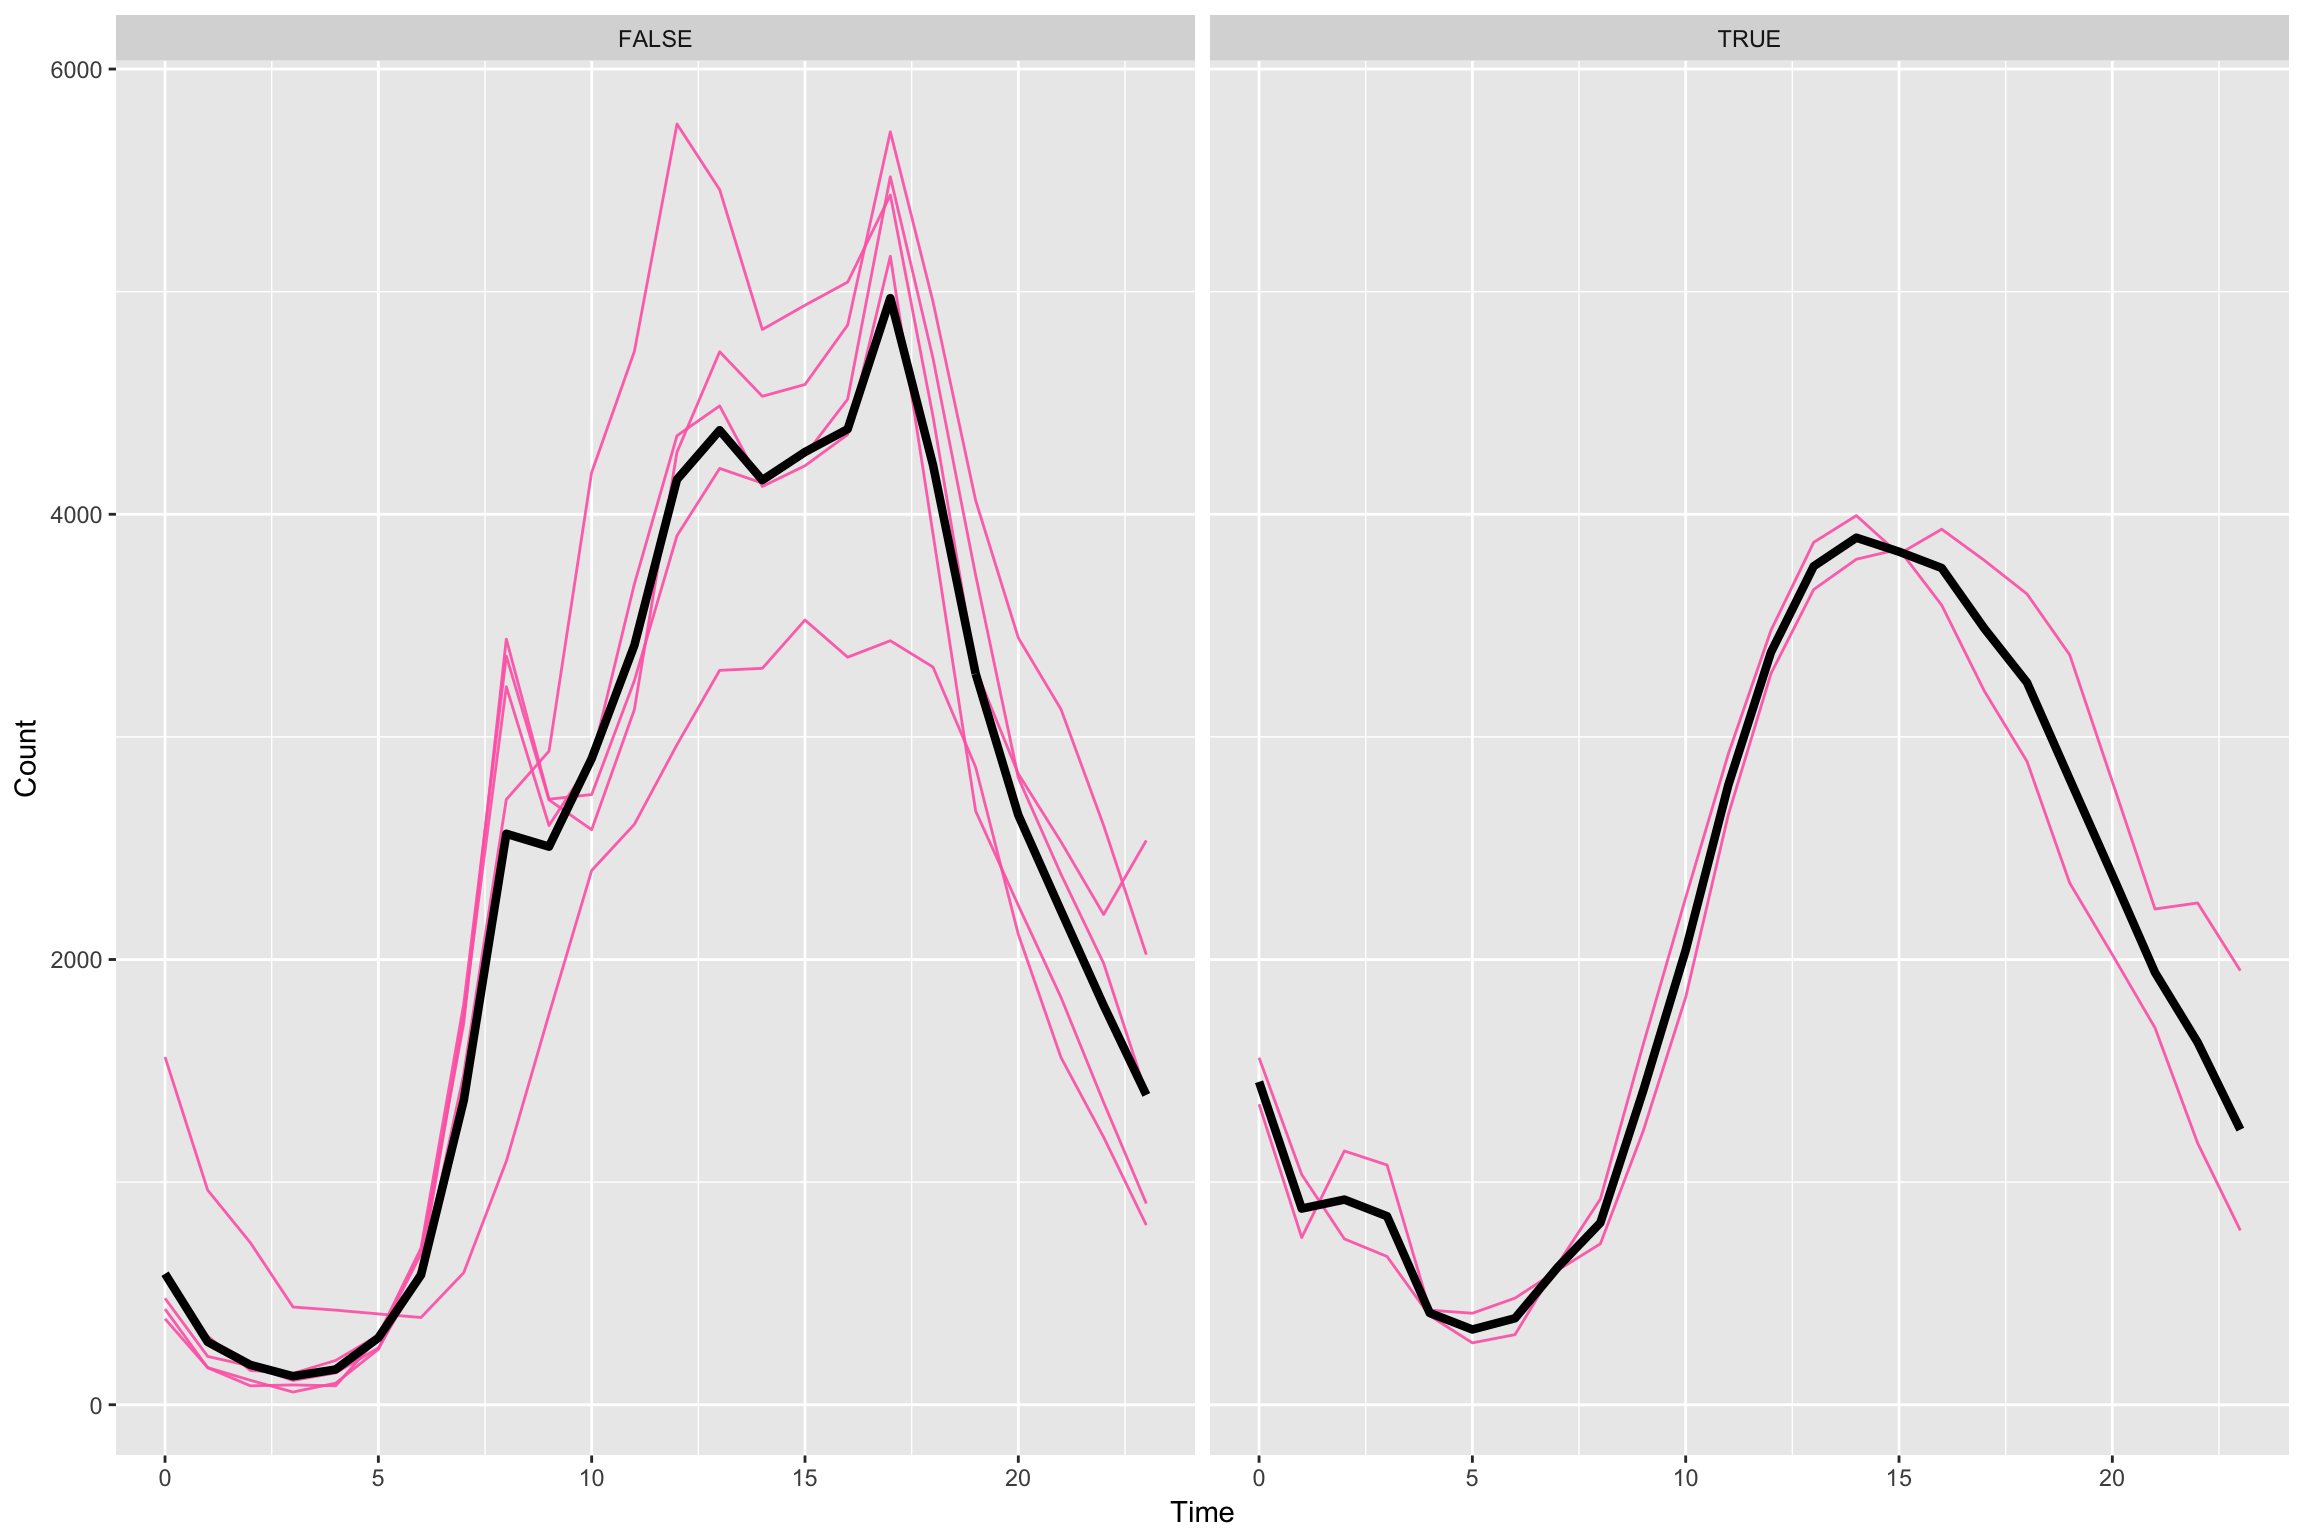
\includegraphics{Submitted_Group_Project_Storyboard_files/figure-latex/unnamed-chunk-10-1} \end{center}

\begin{itemize}
\tightlist
\item
  Russia has had the most players ranked in the top 100 since 2001 with
  314 players
\item
  Australia has had the 9th most with 89
\item
  7 of the countries in the top ten are from Europe
\end{itemize}

\subsection{Predicting players ATP rankings in ten
years}\label{predicting-players-atp-rankings-in-ten-years}

In this section, we will attempt to discover if the ranking of an ATP
player can be predicted to any degree of reliability through looking at
their ranking in the early days of their professional career and their
overall performance in ATP tournaments with a special focus on grand
slams. This section continues to use the deuce package, and the first
thing to do here is to obtain a profile of each player, with their
rankings and some other personal information, such as date of birth.
This is accomplished through the atp\_rankings data set, which is joined
to the atp\_players table, a second table which contains a more fleshed
out version of the players name, date of birth. The result of this join
is displayed below:

\begin{verbatim}
##   ranking_date ranking player_id ranking_points       date first_name
## 1     20000110       1    101736           4135 2000-01-10      Andre
## 2     20000110       2    102338           2915 2000-01-10    Yevgeny
## 3     20000110       3    101948           2419 2000-01-10       Pete
## 4     20000110       4    103017           2184 2000-01-10    Nicolas
## 5     20000110       5    102856           2169 2000-01-10    Gustavo
## 6     20000110       6    102358           2107 2000-01-10     Thomas
##    last_name hand birth_date country_code invalid               name
## 1     Agassi    R   19700429          USA   FALSE       Andre Agassi
## 2 Kafelnikov    R   19740218          RUS   FALSE Yevgeny Kafelnikov
## 3    Sampras    R   19710812          USA   FALSE       Pete Sampras
## 4     Kiefer    R   19770705          GER   FALSE     Nicolas Kiefer
## 5    Kuerten    R   19760910          BRA   FALSE    Gustavo Kuerten
## 6    Enqvist    R   19740313          SWE   FALSE     Thomas Enqvist
##          dob
## 1 1970-04-29
## 2 1974-02-18
## 3 1971-08-12
## 4 1977-07-05
## 5 1976-09-10
## 6 1974-03-13
\end{verbatim}

We would now like to split the rankings of players into their ATP
ranking points after the first 3,6,9 months, then 1 through to 5 years
of their arrival on the ATP tour. This is done by taking the ranking
table formed previously, grouping by player, and filtering out all dates
outside the time period of interest (so to determine ATP ranking points
after 6 months, we select the last recorded value of ATP ranking points
after filtering out dates beyond 6 months after their first recorded
date). This results in tables for each of the data sets, which are then
joined together to create a single time breakdown of the progression of
these players ATP ranking points.

\subsubsection{OBTAINING SOME INDICATION GRAND SLAM
PERFORMANCE}\label{obtaining-some-indication-grand-slam-performance}

How players perform in the glamorous and exciting grand slams over the
years may well prove to be a predictor of ranking points after a solid
amount of time competing at the top level (10 years, hopefully). Below
is calculated the number of wins and losses recorded for each player in
grand slams. It is not however, a good idea to split this variable into
similar time frames as the ranking variables above, as some players may
not have even played a grand slam in their first year, or even 2 or 3
years on tour. Therefore, we take this observation after 4 years.

This is found by taking the table provided by the deuce package,
atp\_matches (containing point by point breakdown statistics of many
grand slam matches over the course of history), and joining this data
set with that describing ATP ranking points after 4 years. The date in
this second table provides the cutoff date past which we should not
consider grand slam results. A snippet of the code to produce this
overall data set is shown below:

Separate tables are created for wins and losses in grand slams, and
finally they are joined to create the final data set.

\begin{Shaded}
\begin{Highlighting}[]
\CommentTok{#******************************************4 YEAR GS************************************************************}
\NormalTok{atp_matches <-}\StringTok{ }\KeywordTok{rename}\NormalTok{(atp_matches,}\DataTypeTok{replace =} \KeywordTok{c}\NormalTok{(}\StringTok{"winner_name"}\NormalTok{ =}\StringTok{ "name"}\NormalTok{))}

\NormalTok{tournaments_4yr <-}\StringTok{ }\KeywordTok{join}\NormalTok{(atp_matches, four_year, }\DataTypeTok{by =} \StringTok{"name"}\NormalTok{) }\OperatorTok\StringTok{ }\KeywordTok{select}\NormalTok{(}\KeywordTok{c}\NormalTok{(tourney_name, tourney_level, name, winner_rank, winner_rank_points, loser_name, loser_rank, loser_rank_points, tourney_start_date, date_4yr, rnkng_pnts_4yr))}


\NormalTok{gs_4yr <-}\StringTok{ }\NormalTok{tournaments_4yr }\OperatorTok\StringTok{ }\KeywordTok{filter}\NormalTok{(tourney_level }\OperatorTok{==}\StringTok{ "Grand Slams"}\NormalTok{) }\OperatorTok\StringTok{ }\KeywordTok{group_by}\NormalTok{(name) }\OperatorTok\StringTok{ }\KeywordTok{filter}\NormalTok{(tourney_start_date }\OperatorTok{<=}\StringTok{ }\NormalTok{date_4yr)}
\NormalTok{gs_4yr_wins <-}\StringTok{ }\KeywordTok{count}\NormalTok{(gs_4yr}\OperatorTok{$}\NormalTok{name) }\OperatorTok\StringTok{ }\KeywordTok{rename}\NormalTok{(}\KeywordTok{c}\NormalTok{(}\StringTok{"x"}\NormalTok{ =}\StringTok{ "name"}\NormalTok{, }\StringTok{"freq"}\NormalTok{ =}\StringTok{ "gs_wins"}\NormalTok{))}
\NormalTok{gs_4yr_wins <-}\StringTok{ }\KeywordTok{join}\NormalTok{(gs_4yr_wins, four_year, }\DataTypeTok{by =} \StringTok{"name"}\NormalTok{) }\OperatorTok\StringTok{ }\KeywordTok{separate}\NormalTok{(date_4yr, }\DataTypeTok{into =} \KeywordTok{c}\NormalTok{(}\StringTok{"year_4yr"}\NormalTok{, }\StringTok{"month_4yr"}\NormalTok{, }\StringTok{"day_4yr"}\NormalTok{)) }\OperatorTok\StringTok{ }\KeywordTok{select}\NormalTok{(name, gs_wins)}


\NormalTok{gs_4yr <-}\StringTok{ }\NormalTok{tournaments_4yr }\OperatorTok\StringTok{ }\KeywordTok{filter}\NormalTok{(tourney_level }\OperatorTok{==}\StringTok{ "Grand Slams"}\NormalTok{) }\OperatorTok\StringTok{ }\KeywordTok{group_by}\NormalTok{(loser_name) }\OperatorTok\StringTok{ }\KeywordTok{filter}\NormalTok{(tourney_start_date }\OperatorTok{<=}\StringTok{ }\NormalTok{date_4yr)}
\NormalTok{gs_4yr_losses <-}\StringTok{ }\KeywordTok{count}\NormalTok{(gs_4yr}\OperatorTok{$}\NormalTok{loser_name) }\OperatorTok\StringTok{ }\KeywordTok{rename}\NormalTok{(}\KeywordTok{c}\NormalTok{(}\StringTok{"x"}\NormalTok{ =}\StringTok{ "name"}\NormalTok{, }\StringTok{"freq"}\NormalTok{ =}\StringTok{ "gs_losses"}\NormalTok{))}
\NormalTok{gs_4yr_losses <-}\StringTok{ }\KeywordTok{join}\NormalTok{(gs_4yr_losses, four_year, }\DataTypeTok{by =} \StringTok{"name"}\NormalTok{) }\OperatorTok\StringTok{ }\KeywordTok{separate}\NormalTok{(date_4yr, }\DataTypeTok{into =} \KeywordTok{c}\NormalTok{(}\StringTok{"year_4yr"}\NormalTok{, }\StringTok{"month_4yr"}\NormalTok{, }\StringTok{"day_4yr"}\NormalTok{)) }\OperatorTok\StringTok{ }\KeywordTok{select}\NormalTok{(name, gs_losses)}


\NormalTok{gs_4yr_wlr <-}\StringTok{ }\KeywordTok{join}\NormalTok{(gs_4yr_losses, gs_4yr_wins, }\DataTypeTok{by =} \StringTok{"name"}\NormalTok{)}

\KeywordTok{head}\NormalTok{(gs_4yr_wlr)}
\NormalTok{##               name gs_losses gs_wins}
\NormalTok{## 1 Aaron Krickstein         5      15}
\NormalTok{## 2        Abe Segal         5       2}
\NormalTok{## 3 Adrian Mannarino         2      NA}
\NormalTok{## 4     Adrian Marcu         1      NA}
\NormalTok{## 5    Adrian Voinea         4       5}
\NormalTok{## 6  Adriano Panatta        22      44}
\end{Highlighting}
\end{Shaded}

\subsubsection{OBTAINING OVERALL ATP TOURNAMENT
PERFORMANCE}\label{obtaining-overall-atp-tournament-performance}

In tennis, there is a fair number of players who may do well in
tournaments other than grand slams, but who repeatedly fail to bring it
together on the big stage. (Alexander Zverev and Nick Kyrgios are
debatedly two of those, just to name a few.) We thought it would be good
to include some reference to these other tournaments as indicators of
performance on the ATP tour.

Luckily this information was available in the atp\_matches table once
more, and allowed us to focus on all professional level tournaments
including grand slams. This table was again joined to the four year
ranking table, or the same reason as it was in the previous step
(obtaining grand slam performance). Four years was chosen as the cutoff
again, to make the wins and losses obtained here comparable to those of
the grand slam data.

\begin{verbatim}
## 'data.frame':    14729 obs. of  10 variables:
##  $ name             : chr  "A Benson" "A Escofet" "A Hall" "A Macdonald" ...
##  $ rnkng_pnts_3mnths: chr  "0" "0" "0" "1" ...
##  $ rnkng_pnts_6mnths: chr  "0" "0" "0" "1" ...
##  $ rnkng_pnts_9mnths: chr  "0" "0" "0" "1" ...
##  $ rnkng_pnts_1yr   : chr  "0" "0" "0" "1" ...
##  $ rnkng_pnts_2yr   : chr  "0" "0" "0" "1" ...
##  $ rnkng_pnts_3yr   : chr  "0" "0" "0" "1" ...
##  $ rnkng_pnts_4yr   : chr  "0" "0" "0" "1" ...
##  $ rnkng_pnts_5yr   : chr  "0" "0" "0" "1" ...
##  $ rnkng_pnts_10yr  : chr  "0" "0" "0" "1" ...
##          name rnkng_pnts_3mnths rnkng_pnts_6mnths rnkng_pnts_9mnths
## 1    A Benson                 0                 0                 0
## 2   A Escofet                 0                 0                 0
## 3      A Hall                 0                 0                 0
## 4 A Macdonald                 1                 1                 1
## 5    A Noffat                 0                 0                 0
## 6    A Uehara                 0                 0                 0
##   rnkng_pnts_1yr rnkng_pnts_2yr rnkng_pnts_3yr rnkng_pnts_4yr
## 1              0              0              0              0
## 2              0              0              0              0
## 3              0              0              0              0
## 4              1              1              1              1
## 5              0              0              0              0
## 6              0              0              0              0
##   rnkng_pnts_5yr rnkng_pnts_10yr
## 1              0               0
## 2              0               0
## 3              0               0
## 4              1               1
## 5              0               0
## 6              0               0
\end{verbatim}

Having obtained this data we could now join the atp tournaments, grand
slams and ranking statistics and combine them all in one table, shown
below.

\begin{Shaded}
\begin{Highlighting}[]
\NormalTok{##join atp tournament performance to ranking data}
\NormalTok{ranking_variables_distinct <-}\StringTok{ }\KeywordTok{merge}\NormalTok{(ranking_variables, atp, }\DataTypeTok{by =} \StringTok{"name"}\NormalTok{)}


\NormalTok{##have to do this joining BEFORE ADJUSTING FOR DUPLICATES}
\NormalTok{ranking_variables_distinct <-}\StringTok{ }\KeywordTok{merge}\NormalTok{(ranking_variables_distinct, gs_4yr_wlr, }\DataTypeTok{by =} \StringTok{"name"}\NormalTok{)}


\KeywordTok{head}\NormalTok{(ranking_variables_distinct)}
\NormalTok{##               name rnkng_pnts_3mnths rnkng_pnts_6mnths rnkng_pnts_9mnths}
\NormalTok{## 1 Aaron Krickstein                 0                 0                 0}
\NormalTok{## 2        Abe Segal                 0                 0                 0}
\NormalTok{## 3 Adrian Mannarino                 4                 4                 7}
\NormalTok{## 4     Adrian Marcu                 0                 0                 0}
\NormalTok{## 5    Adrian Voinea                 2                 2                28}
\NormalTok{## 6  Adriano Panatta                 0                 0                 0}
\NormalTok{##   rnkng_pnts_1yr rnkng_pnts_2yr rnkng_pnts_3yr rnkng_pnts_4yr}
\NormalTok{## 1              0              0              0              0}
\NormalTok{## 2              0              0              0              0}
\NormalTok{## 3              5             60             82            340}
\NormalTok{## 4              0              0              0              0}
\NormalTok{## 5             57             50            150            724}
\NormalTok{## 6              0              0              0              0}
\NormalTok{##   rnkng_pnts_5yr rnkng_pnts_10yr atp_wins atp_losses gs_losses gs_wins}
\NormalTok{## 1              0               0      122         47         5      15}
\NormalTok{## 2              0               0        2          6         5       2}
\NormalTok{## 3            391             729        3          6         2      NA}
\NormalTok{## 4              0              22        2          7         1      NA}
\NormalTok{## 5            885             410       17         30         4       5}
\NormalTok{## 6              0               0      245        158        22      44}
\end{Highlighting}
\end{Shaded}

The data set contained some duplicate rows as some players had identical
names! This was dealt with by adjusting the players name each time it
came up, adding an incrementing number to the end of it e.g.~William
Brown 1, William Brown 2 etc, if there were multiple instances of
William Brown for some reason.

\begin{verbatim}
## 'data.frame':    1089 obs. of  14 variables:
##  $ name             : chr  "Aaron Krickstein" "Abe Segal" "Adrian Mannarino" "Adrian Marcu" ...
##  $ rnkng_pnts_3mnths: chr  "0" "0" "4" "0" ...
##  $ rnkng_pnts_6mnths: chr  "0" "0" "4" "0" ...
##  $ rnkng_pnts_9mnths: chr  "0" "0" "7" "0" ...
##  $ rnkng_pnts_1yr   : chr  "0" "0" "5" "0" ...
##  $ rnkng_pnts_2yr   : chr  "0" "0" "60" "0" ...
##  $ rnkng_pnts_3yr   : chr  "0" "0" "82" "0" ...
##  $ rnkng_pnts_4yr   : chr  "0" "0" "340" "0" ...
##  $ rnkng_pnts_5yr   : chr  "0" "0" "391" "0" ...
##  $ rnkng_pnts_10yr  : chr  "0" "0" "729" "22" ...
##  $ atp_wins         : int  122 2 3 2 17 245 3 4 3 27 ...
##  $ atp_losses       : int  47 6 6 7 30 158 14 4 9 9 ...
##  $ gs_losses        : int  5 5 2 1 4 22 1 1 1 1 ...
##  $ gs_wins          : int  15 2 NA NA 5 44 1 NA NA 3 ...
\end{verbatim}

\subsubsection{PCA ANALYSIS ON THE VARIABLES ON THIS
DATASET}\label{pca-analysis-on-the-variables-on-this-dataset}

In this section we conduct principal component analysis on all the
variables in this data set. This will allow us to identify which
variables are intercorrelated, and which of them are most important in
explaining variation among them. The variables will be separated into
principal components which will highlight the most important information
in the data set.

The first step here is to take our data set and remove the name column,
then format all the other variables as numeric, a key condition for PCA.

\begin{verbatim}
## 'data.frame':    1089 obs. of  13 variables:
##  $ rnkng_pnts_3mnths: num  0 0 4 0 2 0 0 0 0 0 ...
##  $ rnkng_pnts_6mnths: num  0 0 4 0 2 0 57 0 0 0 ...
##  $ rnkng_pnts_9mnths: num  0 0 7 0 28 0 57 0 0 0 ...
##  $ rnkng_pnts_1yr   : num  0 0 5 0 57 0 48 0 0 0 ...
##  $ rnkng_pnts_2yr   : num  0 0 60 0 50 0 156 0 0 0 ...
##  $ rnkng_pnts_3yr   : num  0 0 82 0 150 0 260 0 0 458 ...
##  $ rnkng_pnts_4yr   : num  0 0 340 0 724 0 281 0 0 261 ...
##  $ rnkng_pnts_5yr   : num  0 0 391 0 885 0 611 74 0 42 ...
##  $ rnkng_pnts_10yr  : num  0 0 729 22 410 0 547 12 0 1 ...
##  $ atp_wins         : num  122 2 3 2 17 245 3 4 3 27 ...
##  $ atp_losses       : num  47 6 6 7 30 158 14 4 9 9 ...
##  $ gs_losses        : num  5 5 2 1 4 22 1 1 1 1 ...
##  $ gs_wins          : num  15 2 NA NA 5 44 1 NA NA 3 ...
## 'data.frame':    1089 obs. of  12 variables:
##  $ rnkng_pnts_6mnths: num  0 0 4 0 2 0 57 0 0 0 ...
##  $ rnkng_pnts_9mnths: num  0 0 7 0 28 0 57 0 0 0 ...
##  $ rnkng_pnts_1yr   : num  0 0 5 0 57 0 48 0 0 0 ...
##  $ rnkng_pnts_2yr   : num  0 0 60 0 50 0 156 0 0 0 ...
##  $ rnkng_pnts_3yr   : num  0 0 82 0 150 0 260 0 0 458 ...
##  $ rnkng_pnts_4yr   : num  0 0 340 0 724 0 281 0 0 261 ...
##  $ rnkng_pnts_5yr   : num  0 0 391 0 885 0 611 74 0 42 ...
##  $ rnkng_pnts_10yr  : num  0 0 729 22 410 0 547 12 0 1 ...
##  $ atp_wins         : num  122 2 3 2 17 245 3 4 3 27 ...
##  $ atp_losses       : num  47 6 6 7 30 158 14 4 9 9 ...
##  $ gs_losses        : num  5 5 2 1 4 22 1 1 1 1 ...
##  $ gs_wins          : num  15 2 NA NA 5 44 1 NA NA 3 ...
##   rnkng_pnts_6mnths rnkng_pnts_9mnths rnkng_pnts_1yr rnkng_pnts_2yr
## 1                 0                 0              0              0
## 2                 0                 0              0              0
## 3                 4                 7              5             60
## 4                 0                 0              0              0
## 5                 2                28             57             50
## 6                 0                 0              0              0
##   rnkng_pnts_3yr rnkng_pnts_4yr rnkng_pnts_5yr rnkng_pnts_10yr atp_wins
## 1              0              0              0               0      122
## 2              0              0              0               0        2
## 3             82            340            391             729        3
## 4              0              0              0              22        2
## 5            150            724            885             410       17
## 6              0              0              0               0      245
##   atp_losses gs_losses gs_wins
## 1         47         5      15
## 2          6         5       2
## 3          6         2      NA
## 4          7         1      NA
## 5         30         4       5
## 6        158        22      44
\end{verbatim}

\subsubsection{DATA STANDARDISATION}\label{data-standardisation}

In principal component analysis, variables are often scaled
(i.e.~standardized). This is a good idea when variables are measured in
different scales (e.g: kilograms, kilometers, centimeters, \ldots{});
otherwise, the PCA outputs obtained will be severely affected.

The goal here is to make the variables comparable. Generally variables
are scaled to have: i) standard deviation one and ii) mean zero The
function PCA() {[}FactoMineR package{]} can be used.

This standardization to the same scale avoids some variables to become
dominant just because of their large measurement units. It makes
variable comparable.

The R code below, computes principal component analysis on the active
individuals/variables:

\begin{Shaded}
\begin{Highlighting}[]
\KeywordTok{library}\NormalTok{(}\StringTok{"FactoMineR"}\NormalTok{)}
\NormalTok{res.pca1 <-}\StringTok{ }\KeywordTok{PCA}\NormalTok{(ranking_variables_distinct, }\DataTypeTok{graph =} \OtherTok{FALSE}\NormalTok{)}
\KeywordTok{print}\NormalTok{(res.pca1)}
\NormalTok{## **Results for the Principal Component Analysis (PCA)**}
\NormalTok{## The analysis was performed on 1089 individuals, described by 12 variables}
\NormalTok{## *The results are available in the following objects:}
\NormalTok{## }
\NormalTok{##    name               description                          }
\NormalTok{## 1  "$eig"             "eigenvalues"                        }
\NormalTok{## 2  "$var"             "results for the variables"          }
\NormalTok{## 3  "$var$coord"       "coord. for the variables"           }
\NormalTok{## 4  "$var$cor"         "correlations variables - dimensions"}
\NormalTok{## 5  "$var$cos2"        "cos2 for the variables"             }
\NormalTok{## 6  "$var$contrib"     "contributions of the variables"     }
\NormalTok{## 7  "$ind"             "results for the individuals"        }
\NormalTok{## 8  "$ind$coord"       "coord. for the individuals"         }
\NormalTok{## 9  "$ind$cos2"        "cos2 for the individuals"           }
\NormalTok{## 10 "$ind$contrib"     "contributions of the individuals"   }
\NormalTok{## 11 "$call"            "summary statistics"                 }
\NormalTok{## 12 "$call$centre"     "mean of the variables"              }
\NormalTok{## 13 "$call$ecart.type" "standard error of the variables"    }
\NormalTok{## 14 "$call$row.w"      "weights for the individuals"        }
\NormalTok{## 15 "$call$col.w"      "weights for the variables"}
\end{Highlighting}
\end{Shaded}

\subsubsection{VISUALIZATION AND
INTERPRETATION}\label{visualization-and-interpretation}

We will use the factoextra R package to help in the interpretation of
PCA.

Eigenvalues / Variances The eigenvalues measure the amount of variation
retained by each principal component in the data set. Eigenvalues are
large for the first PCs and small for the subsequent PCs. That is, the
first PCs corresponds to the directions with the maximum amount of
variation in the data set.

We examine the eigenvalues to determine the number of principal
components to be considered. The eigenvalues and the proportion of
variances (i.e., information) retained by the principal components (PCs)
can be extracted using the function get\_eigenvalue() from the
factoextra package.

\begin{verbatim}
##        eigenvalue variance.percent cumulative.variance.percent
## Dim.1  5.50886318       45.9071932                    45.90719
## Dim.2  3.19194422       26.5995352                    72.50673
## Dim.3  1.29124833       10.7604028                    83.26713
## Dim.4  0.52624329        4.3853607                    87.65249
## Dim.5  0.49032933        4.0860777                    91.73857
## Dim.6  0.27878221        2.3231851                    94.06175
## Dim.7  0.22789740        1.8991450                    95.96090
## Dim.8  0.13433485        1.1194571                    97.08036
## Dim.9  0.12205968        1.0171640                    98.09752
## Dim.10 0.09557539        0.7964616                    98.89398
## Dim.11 0.07987972        0.6656643                    99.55965
## Dim.12 0.05284239        0.4403533                   100.00000
\end{verbatim}

Eigenvalues can be used to determine the number of principal components
to retain after PCA (Kaiser 1961):

An eigenvalue \textgreater{} 1 indicates that PCs account for more
variance than accounted by one of the original variables in standardized
data. This is commonly used as a cutoff point for which PCs are
retained. This is true only when the data is standardized.

You can also limit the number of components to a number that accounts
for a certain fraction of the total variance. So for example here, as
can be seen from the eigen values above, we might choose to stop at
dimension 7, as up to this point, 95\% of the variation is explained.

\subsubsection{SCREE PLOT}\label{scree-plot}

An alternative method to determine the number of principal components is
to look at a Scree Plot, which is the plot of eigenvalues ordered from
largest to the smallest. The number of component is determined at the
point, beyond which the remaining eigenvalues are all relatively small
and of comparable size (Jollife 2002, Peres-Neto, Jackson, and Somers
(2005)).

The scree plot can be produced using the function fviz\_eig() or
fviz\_screeplot() from the factoextra package.

\begin{center}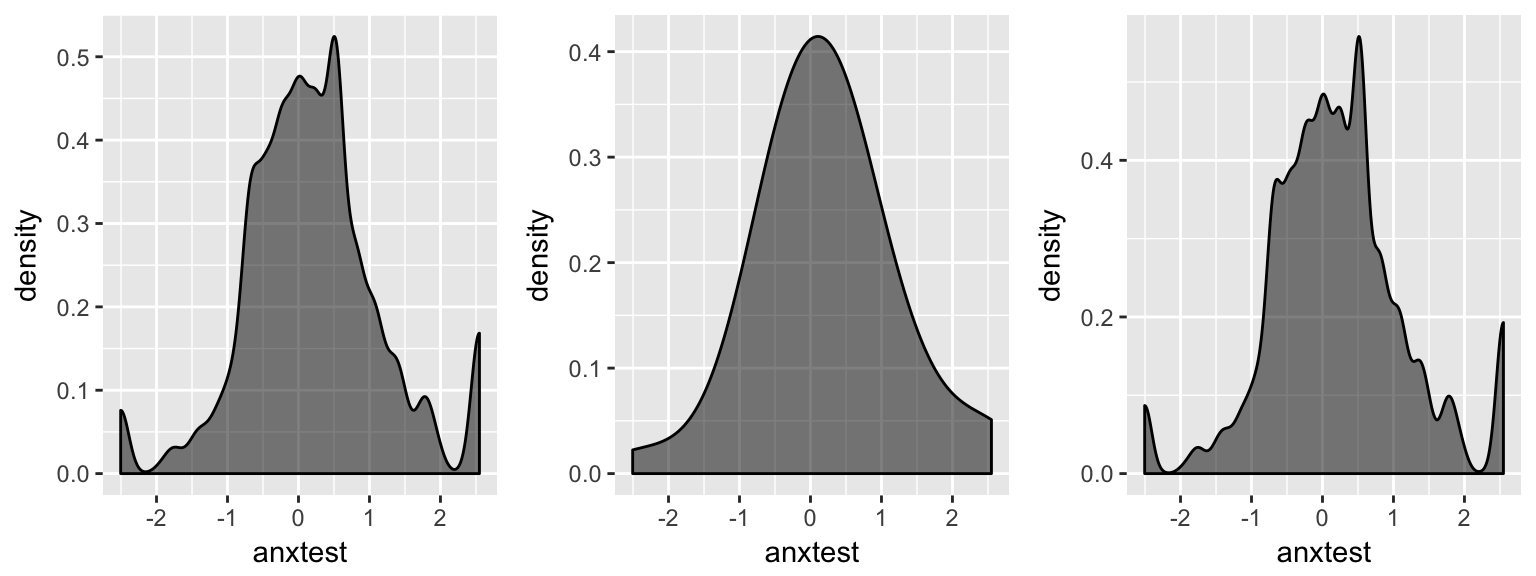
\includegraphics{Submitted_Group_Project_Storyboard_files/figure-latex/unnamed-chunk-25-1} \end{center}

From the plot above, we might want to stop at the 7th principal
component. 95\% of the information (variances) contained in the data are
retained by the first five principal components.PUT RIGHT VALUES IN

\subsubsection{RESULTS}\label{results}

To extract the results for variables from a PCA output we can use the
function get\_pca\_var() (factoextra package). This function provides a
list of matrices containing all the results for the active variables
(coordinates, correlation between variables and axes, squared cosine and
contributions)

The components of the get\_pca\_var() can be used in the plot of our
variables as follows:

var\(coord: coordinates of variables to create a scatter plot var\)cos2:
represents the quality of representation for variables on the factor
map. It's calculated as the squared coordinates: var.cos2 = var.coord *
var.coord. var\$contrib: contains the contributions (in percentage) of
the variables to the principal components. The contribution of a
variable (var) to a given principal component is (in percentage) :
(var.cos2 * 100) / (total cos2 of the component).

\begin{verbatim}
## Principal Component Analysis Results for variables
##  ===================================================
##   Name       Description                                    
## 1 "$coord"   "Coordinates for the variables"                
## 2 "$cor"     "Correlations between variables and dimensions"
## 3 "$cos2"    "Cos2 for the variables"                       
## 4 "$contrib" "contributions of the variables"
##                       Dim.1      Dim.2      Dim.3        Dim.4
## rnkng_pnts_6mnths 0.7396830 0.06636937  0.5356839  0.183535865
## rnkng_pnts_9mnths 0.8003324 0.07234540  0.5316438  0.097870521
## rnkng_pnts_1yr    0.8290986 0.08838776  0.4255562 -0.002166276
## rnkng_pnts_2yr    0.8603207 0.15971845 -0.0469459 -0.260805001
## rnkng_pnts_3yr    0.8709076 0.14336455 -0.1810676 -0.268405180
## rnkng_pnts_4yr    0.8767204 0.13948107 -0.3413019 -0.027754990
##                          Dim.5
## rnkng_pnts_6mnths -0.083898074
## rnkng_pnts_9mnths -0.055824477
## rnkng_pnts_1yr     0.005418478
## rnkng_pnts_2yr     0.185113611
## rnkng_pnts_3yr     0.166862814
## rnkng_pnts_4yr     0.061171122
##                       Dim.1       Dim.2       Dim.3        Dim.4
## rnkng_pnts_6mnths 0.5471309 0.004404894 0.286957200 3.368541e-02
## rnkng_pnts_9mnths 0.6405320 0.005233857 0.282645175 9.578639e-03
## rnkng_pnts_1yr    0.6874045 0.007812396 0.181098086 4.692751e-06
## rnkng_pnts_2yr    0.7401516 0.025509985 0.002203917 6.801925e-02
## rnkng_pnts_3yr    0.7584800 0.020553394 0.032785471 7.204134e-02
## rnkng_pnts_4yr    0.7686386 0.019454968 0.116487020 7.703395e-04
##                          Dim.5
## rnkng_pnts_6mnths 0.0070388868
## rnkng_pnts_9mnths 0.0031163722
## rnkng_pnts_1yr    0.0000293599
## rnkng_pnts_2yr    0.0342670488
## rnkng_pnts_3yr    0.0278431986
## rnkng_pnts_4yr    0.0037419062
##                       Dim.1     Dim.2      Dim.3        Dim.4       Dim.5
## rnkng_pnts_6mnths  9.931829 0.1380003 22.2232388 6.401110e+00 1.435542699
## rnkng_pnts_9mnths 11.627299 0.1639708 21.8892964 1.820192e+00 0.635567175
## rnkng_pnts_1yr    12.478155 0.2447535 14.0250393 8.917456e-04 0.005987792
## rnkng_pnts_2yr    13.435651 0.7991990  0.1706811 1.292544e+01 6.988578295
## rnkng_pnts_3yr    13.768358 0.6439146  2.5390523 1.368974e+01 5.678468970
## rnkng_pnts_4yr    13.952762 0.6095021  9.0212716 1.463847e-01 0.763141420
\end{verbatim}

\subsubsection{CORRELATION CIRCLE}\label{correlation-circle}

The correlation between a variable and a principal component (PC) is
used as the coordinates of the variable on the PC. The representation of
variables differs from the plot of the observations: The observations
are represented by their projections, but the variables are represented
by their correlations (Abdi and Williams 2010). Color by cos2 values:
quality on the factor map

\begin{center}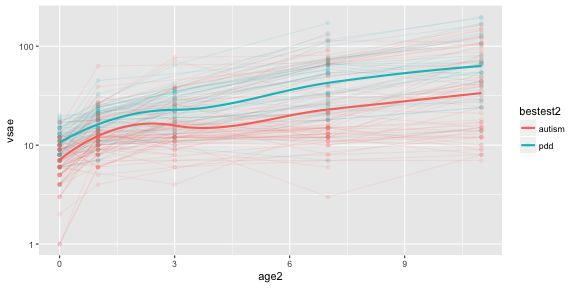
\includegraphics{Submitted_Group_Project_Storyboard_files/figure-latex/unnamed-chunk-27-1} \end{center}

The plot above is also known as variable correlation plots. It shows the
relationships between all variables. It can be interpreted as follows:

Positively correlated variables are grouped together. We can see that
atp\_wins and gs\_wins are correlated, as well as atp\_losses and
gs\_losses. This makes sense, as players who do well in most atp
tournaments will tend to also perform in the grand slams, although there
are some outliers as mentioned previously. Negatively correlated
variables are positioned on opposite sides of the plot origin (opposed
quadrants). Interestingly, ranking points and tournament performance are
not correlated, from this data. This is somewhat counter intuitive, as
one would suspect that good tournament performance would result in
better ranks. However, there would be some players who do well in
tournaments which don't offer a high number of ranking points, which
would explain why tournament performance and ranking points are not
really correlated here.

The distance between variables and the origin measures the quality of
the variables on the factor map. Variables that are away from the origin
are well represented on the factor map. Due to the cluster of variables
on this correlation plot, it is hard to see the quality for each
variable. The cos2 on the key of this plot is explained below.

\subsubsection{QUALITY OF
REPRESENTATION}\label{quality-of-representation}

The quality of representation of the variables on factor map is called
cos2 (square cosine, squared coordinates).

A high cos2 indicates a good representation of the variable on the
principal component. In this case the variable is positioned close to
the circumference of the correlation circle.

A low cos2 indicates that the variable is not perfectly represented by
the PCs. In this case the variable is close to the center of the circle.

\begin{verbatim}
##                       Dim.1       Dim.2       Dim.3        Dim.4
## rnkng_pnts_6mnths 0.5471309 0.004404894 0.286957200 3.368541e-02
## rnkng_pnts_9mnths 0.6405320 0.005233857 0.282645175 9.578639e-03
## rnkng_pnts_1yr    0.6874045 0.007812396 0.181098086 4.692751e-06
## rnkng_pnts_2yr    0.7401516 0.025509985 0.002203917 6.801925e-02
##                          Dim.5
## rnkng_pnts_6mnths 0.0070388868
## rnkng_pnts_9mnths 0.0031163722
## rnkng_pnts_1yr    0.0000293599
## rnkng_pnts_2yr    0.0342670488
\end{verbatim}

\begin{center}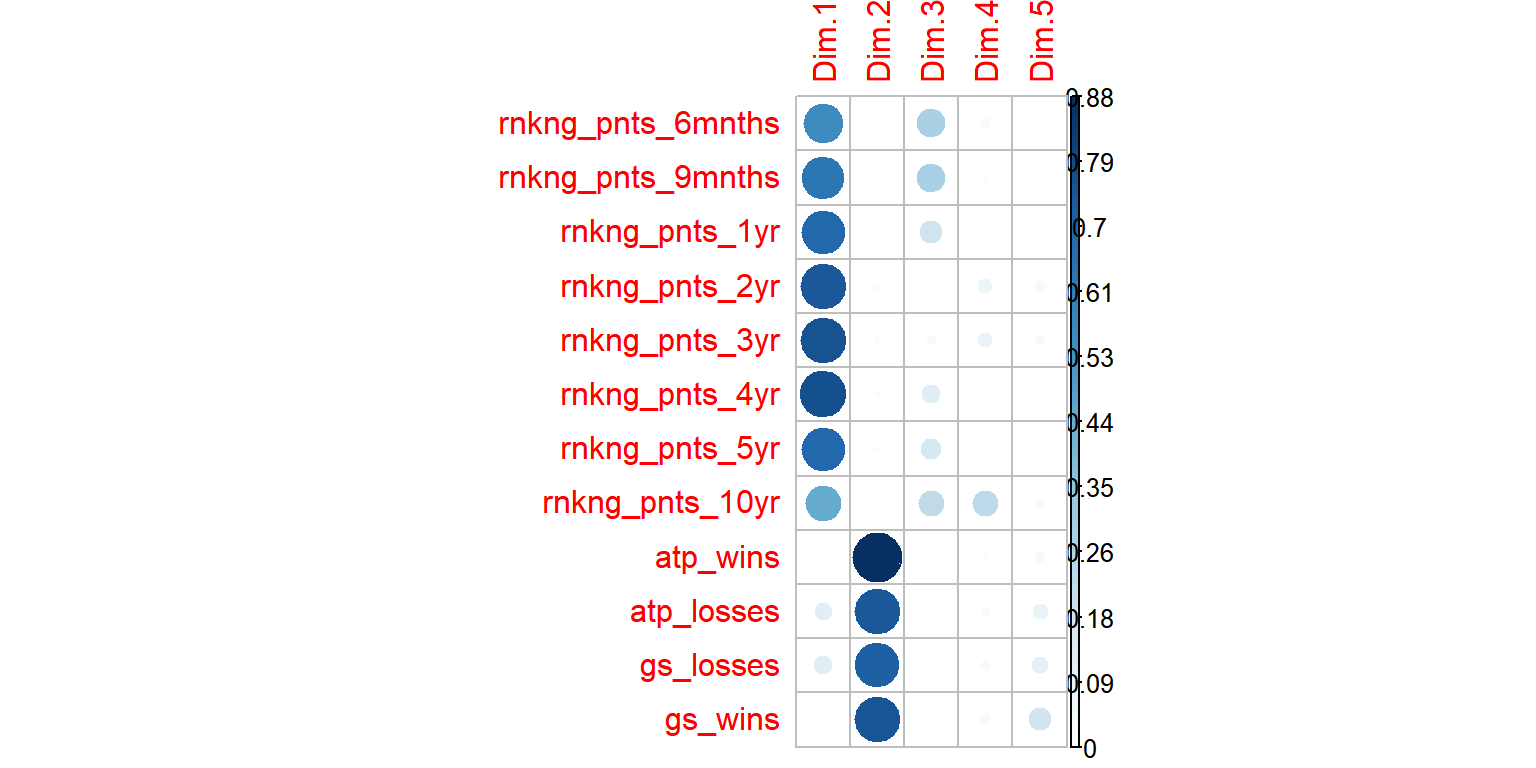
\includegraphics{Submitted_Group_Project_Storyboard_files/figure-latex/unnamed-chunk-28-1} \end{center}

A bar chart of the cos2 is probably a more user-friendly result:

\begin{center}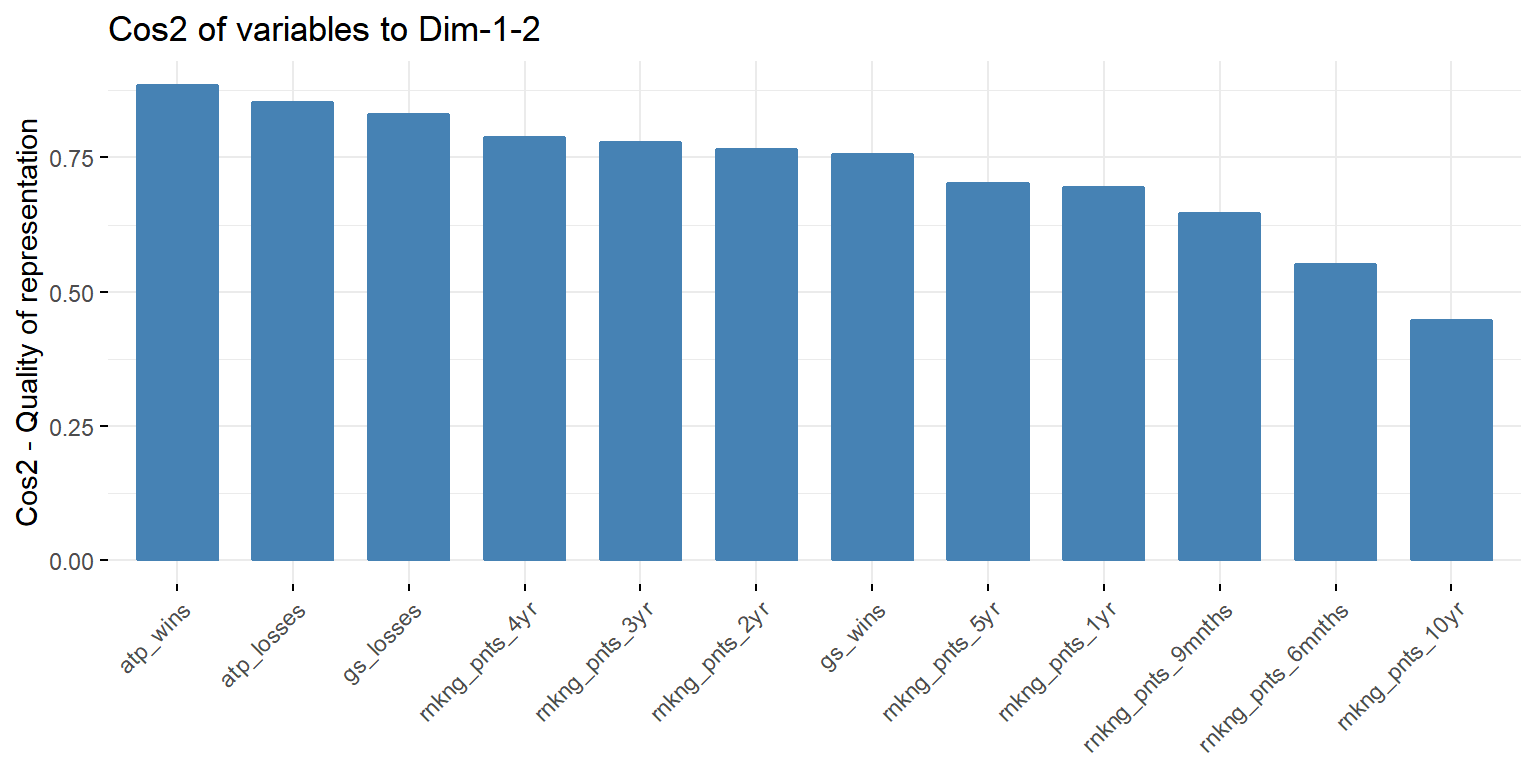
\includegraphics{Submitted_Group_Project_Storyboard_files/figure-latex/unnamed-chunk-29-1} \end{center}

Contributions of variables to PCs The contributions of variables in
accounting for the variability in a given principal component are
expressed in percentage.

Variables that are correlated with PC1 (i.e., Dim.1) and PC2 (i.e.,
Dim.2) are the most important in explaining the variability in the data
set. Variables that are not correlated with any PC or correlated with
the last dimensions are variables with low contribution and might be
removed to simplify the overall analysis. The larger the value of the
contribution, the more the variable contributes to the component.

\begin{verbatim}
##                       Dim.1     Dim.2      Dim.3        Dim.4       Dim.5
## rnkng_pnts_6mnths  9.931829 0.1380003 22.2232388 6.401110e+00 1.435542699
## rnkng_pnts_9mnths 11.627299 0.1639708 21.8892964 1.820192e+00 0.635567175
## rnkng_pnts_1yr    12.478155 0.2447535 14.0250393 8.917456e-04 0.005987792
## rnkng_pnts_2yr    13.435651 0.7991990  0.1706811 1.292544e+01 6.988578295
\end{verbatim}

\begin{center}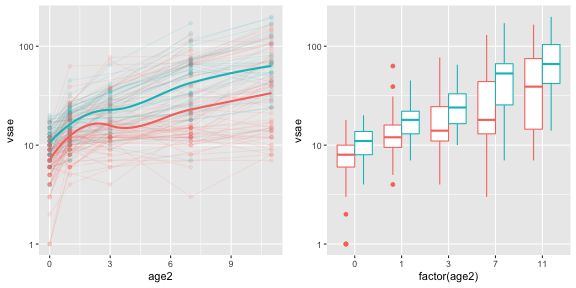
\includegraphics{Submitted_Group_Project_Storyboard_files/figure-latex/unnamed-chunk-31-1} \end{center}

Once again bar charts is also helpful to visualise which variables are
contributing most to the variations. Here are the contributions of each
variable to PC1.

\begin{center}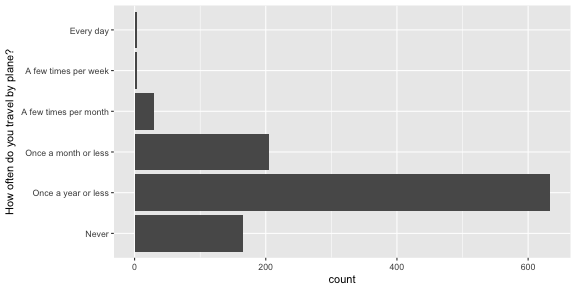
\includegraphics{Submitted_Group_Project_Storyboard_files/figure-latex/unnamed-chunk-32-1} \end{center}

Likewise the contributions to PC2

\begin{center}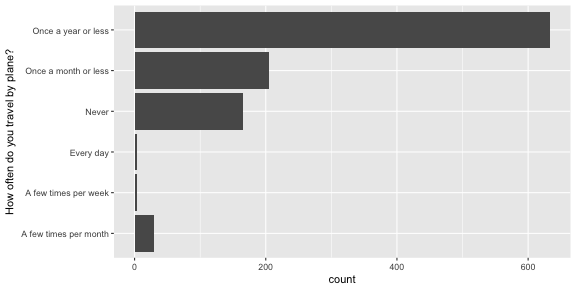
\includegraphics{Submitted_Group_Project_Storyboard_files/figure-latex/unnamed-chunk-33-1} \end{center}

Now the total contribution to PC1 and PC2

\begin{center}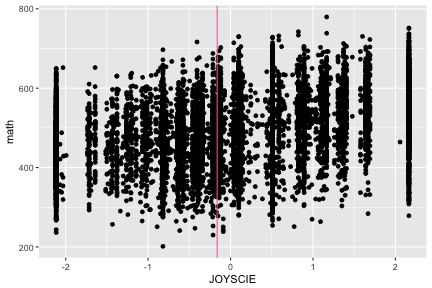
\includegraphics{Submitted_Group_Project_Storyboard_files/figure-latex/unnamed-chunk-34-1} \end{center}

Clearly these plots confirm the information plotted in the correlation
circle above. The ranking points are correlated with Dim 1 and
tournament performance to Dim2.

The red dashed line on the graphs above indicate the expected average
contribution.

\subsubsection{LINEAR REGRESSION TO PREDICT RANKING AT TEN YEAR
MARK}\label{linear-regression-to-predict-ranking-at-ten-year-mark}

We will now perform multiple linear regression to determine the
contributions of different variables to rnkng\_pnts\_10yr, the outcome
variable here.

The first model takes into account all possible variables, with ranking
points at ten years as the outcome.

\begin{verbatim}
## 
## Call:
## lm(formula = rnkng_pnts_10yr ~ rnkng_pnts_6mnths + rnkng_pnts_9mnths + 
##     rnkng_pnts_1yr + rnkng_pnts_2yr + rnkng_pnts_3yr + rnkng_pnts_4yr + 
##     rnkng_pnts_5yr + gs_losses + gs_wins + atp_wins + atp_losses, 
##     data = ranking_variables_distinct)
## 
## Residuals:
##     Min      1Q  Median      3Q     Max 
## -3416.0   -49.6   -36.2    -3.5  6816.2 
## 
## Coefficients:
##                   Estimate Std. Error t value Pr(>|t|)    
## (Intercept)       48.69587   33.81612   1.440 0.150274    
## rnkng_pnts_6mnths  6.98672    2.87544   2.430 0.015338 *  
## rnkng_pnts_9mnths  0.65027    2.80687   0.232 0.816855    
## rnkng_pnts_1yr    -5.08387    1.53472  -3.313 0.000968 ***
## rnkng_pnts_2yr     0.68122    0.32309   2.108 0.035317 *  
## rnkng_pnts_3yr    -0.66500    0.17652  -3.767 0.000178 ***
## rnkng_pnts_4yr     1.00740    0.12186   8.267 6.14e-16 ***
## rnkng_pnts_5yr     0.53293    0.08612   6.189 9.93e-10 ***
## gs_losses          3.88989    8.99951   0.432 0.665694    
## gs_wins           -1.25455    5.11875  -0.245 0.806454    
## atp_wins           0.38167    0.87349   0.437 0.662269    
## atp_losses        -1.08804    1.32196  -0.823 0.410738    
## ---
## Signif. codes:  0 '***' 0.001 '**' 0.01 '*' 0.05 '.' 0.1 ' ' 1
## 
## Residual standard error: 569.1 on 759 degrees of freedom
##   (318 observations deleted due to missingness)
## Multiple R-squared:  0.5443, Adjusted R-squared:  0.5376 
## F-statistic:  82.4 on 11 and 759 DF,  p-value: < 2.2e-16
\end{verbatim}

Clearly ranking points at 6 months, and tournament results are quite
insignificant here, indicating that as one might expect, ranking can
only be loosely predicted by previous rankings at around 5 or 6 years
prior to the current date. The R squared value of this regression is a
weak 0.5376, telling us that predicting will be unreliable at the best
of times.

We will now remove the variables which don't contribute to the
prediction, and build a new model.

\begin{verbatim}
## 
## Call:
## lm(formula = rnkng_pnts_10yr ~ rnkng_pnts_1yr + rnkng_pnts_2yr + 
##     rnkng_pnts_3yr + rnkng_pnts_4yr + rnkng_pnts_5yr, data = ranking_variables_distinct)
## 
## Residuals:
##     Min      1Q  Median      3Q     Max 
## -3382.3   -49.1   -49.1   -49.1  6998.3 
## 
## Coefficients:
##                Estimate Std. Error t value Pr(>|t|)    
## (Intercept)    49.07364   17.33843   2.830 0.004736 ** 
## rnkng_pnts_1yr -2.03759    0.76367  -2.668 0.007741 ** 
## rnkng_pnts_2yr  0.56868    0.27292   2.084 0.037423 *  
## rnkng_pnts_3yr -0.55301    0.15042  -3.676 0.000248 ***
## rnkng_pnts_4yr  0.89055    0.10558   8.435  < 2e-16 ***
## rnkng_pnts_5yr  0.62342    0.07373   8.456  < 2e-16 ***
## ---
## Signif. codes:  0 '***' 0.001 '**' 0.01 '*' 0.05 '.' 0.1 ' ' 1
## 
## Residual standard error: 523.5 on 1083 degrees of freedom
## Multiple R-squared:  0.5146, Adjusted R-squared:  0.5124 
## F-statistic: 229.7 on 5 and 1083 DF,  p-value: < 2.2e-16
\end{verbatim}

Interestingly the model hardly improves, meaning that even though
ranking points in the first 5 years a player is on tour can be somewhat
helpful in predicting where they will be in ten years, it is still
anybody's guess.

It can however be seen that the later ranking points (those at 3, 4 and
5 years) are more significant than earlier ones, so a final regression
model will be constructed, taking only these into account.

\begin{verbatim}
## 
## Call:
## lm(formula = rnkng_pnts_10yr ~ rnkng_pnts_3yr + rnkng_pnts_4yr + 
##     rnkng_pnts_5yr, data = ranking_variables_distinct)
## 
## Residuals:
##     Min      1Q  Median      3Q     Max 
## -3414.6   -44.1   -44.1   -44.1  6993.2 
## 
## Coefficients:
##                Estimate Std. Error t value Pr(>|t|)    
## (Intercept)    44.13758   17.31243   2.549   0.0109 *  
## rnkng_pnts_3yr -0.46959    0.11983  -3.919 9.45e-05 ***
## rnkng_pnts_4yr  0.91851    0.10076   9.115  < 2e-16 ***
## rnkng_pnts_5yr  0.60105    0.07258   8.281 3.55e-16 ***
## ---
## Signif. codes:  0 '***' 0.001 '**' 0.01 '*' 0.05 '.' 0.1 ' ' 1
## 
## Residual standard error: 525.2 on 1085 degrees of freedom
## Multiple R-squared:  0.5107, Adjusted R-squared:  0.5093 
## F-statistic: 377.4 on 3 and 1085 DF,  p-value: < 2.2e-16
\end{verbatim}

Once again, the R squared value does not change, remaining 0.5093.

\subsubsection{CONCLUSIONS}\label{conclusions}

You may be wondering why ranking points at 10 years was chosen as an
outcome variable, as it is highly variable. Surely career high ranking
or cumulative ranking points would have been more informative outcome
variables. The simple answer to this is that there was insufficient data
(not to mention time:) ) to obtain these sort of variables.

Overall however, it is plain that trying to predict the chosen outcome
variable was unreliable at best. Only a few variables which were closer
to the outcome can predict with anything approaching 50\% reliability.

It is perhaps not surprising that trying to predict sport in general is
highly difficult, as if it was able to be predicted easily, there would
be no interest in it. This simply highlights the exciting nature of the
game of tennis, in that matches can change drastically across a couple
of sets of even games or points, and there are so many variables which
contribute the outcome of any one match (location, court surface or
player injury record or status, for example) that it is very hard to
forecast results.

Throughout this analysis it became increasingly evident that one cannot
simply trust data given, and the importance of conducting sanity checks
throughout the analysis cannot be overestimated, both for detecting
errors in ones own analysis and for noticing unrealistic readings in the
supplied data. For example, some of the data sets in the deuce package
contained multiple missing values making analysis unreliable, and
sometimes contained multiple instances of the same player (up to 80
instances of identical players).

\subsection{Left-handed vs Right-handed
players}\label{left-handed-vs-right-handed-players}

\begin{itemize}
\item
  Do Left-handed players have an advantage over Right-handed players in
  the last four years from 2015 to 2018 in ATP?
\item
  There is a saying that left-handed people have an advantage over
  right-handed people.Is it true or not?
\end{itemize}

\subsubsection{Dataset}\label{dataset}

\begin{itemize}
\tightlist
\item
  First we just use atp\_players data set and join to the data set
  atp\_rankings using left\_join by player id to get the ranking data
  and handedness type of player at the same time.
\item
  then unselect ``date'' variable in this data set because it's same as
  ranking\_date.\\
\item
  filter date from 2015 to 2018 for our research.
\end{itemize}

\subsubsection{Average ranking of each
player}\label{average-ranking-of-each-player}

\begin{itemize}
\tightlist
\item
  Because the ranking period of each player is not the same, we take the
  average ranking to analyse whether the handedness type has any effect
  on player ranking.
\item
  Because the data is too large and we only take the latest 4 years from
  2015 to 2018 to calculate average ranking for each handedness type and
  got the data set like it.
\end{itemize}

\begin{verbatim}
## # A tibble: 6,100 x 4
##    player_id    AVE hand   year
##        <int>  <dbl> <chr> <dbl>
##  1    100415  892.  R      2015
##  2    100644   99.4 R      2015
##  3    101339 1879.  R      2015
##  4    102033 1542.  R      2015
##  5    102240 1970.  R      2015
##  6    102506 1289   R      2015
##  7    102703 1296.  R      2015
##  8    102774 1669.  R      2015
##  9    102822 1758.  R      2015
## 10    102863  924   R      2015
## # ... with 6,090 more rows
\end{verbatim}

\subsubsection{Distruibution of Average
ranking.}\label{distruibution-of-average-ranking.}

\begin{itemize}
\tightlist
\item
  We use the box plot to observe the distribution of player's average
  ranking for right hand and left hand.
\end{itemize}

\begin{Shaded}
\begin{Highlighting}[]
\KeywordTok{ggplot}\NormalTok{(atp_htpall,}\KeywordTok{aes}\NormalTok{(}\DataTypeTok{x=}\NormalTok{hand, }\DataTypeTok{y=}\NormalTok{AVE)) }\OperatorTok{+}\StringTok{ }
\StringTok{  }\KeywordTok{geom_boxplot}\NormalTok{() }\OperatorTok{+}
\StringTok{  }\KeywordTok{facet_wrap}\NormalTok{(}\OperatorTok{~}\NormalTok{year)}
\end{Highlighting}
\end{Shaded}

\begin{center}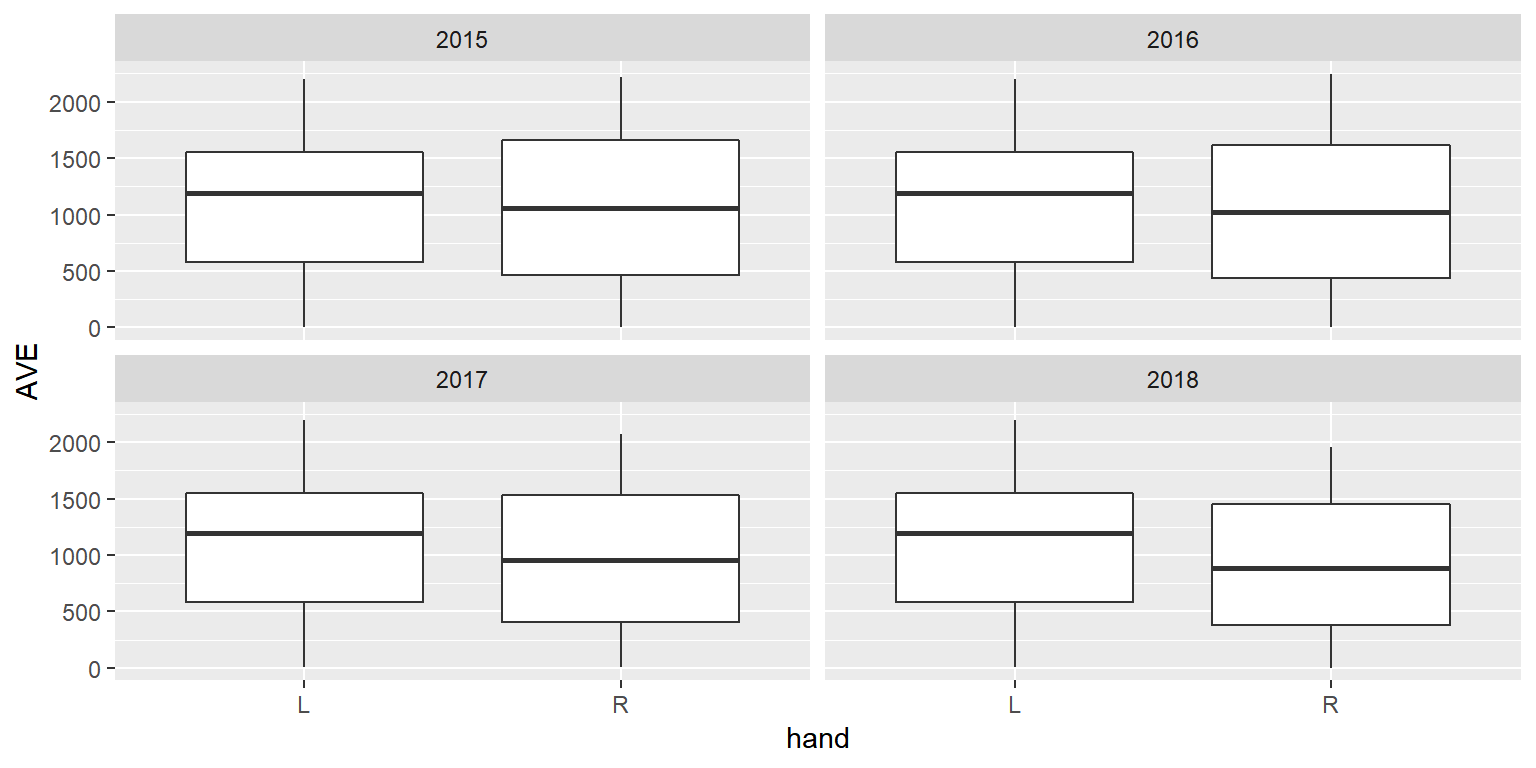
\includegraphics{Submitted_Group_Project_Storyboard_files/figure-latex/unnamed-chunk-40-1} \end{center}

\begin{itemize}
\tightlist
\item
  We can see that the difference between the two handedness type is
  tiny.
\item
  The distribution of left-handed players are worse than right-handed
  players. But it can't be prove that the claim is true or false.
\end{itemize}

\subsubsection{Detailed analyse}\label{detailed-analyse}

\begin{itemize}
\tightlist
\item
  For the detailed analyse, we create a subset to compare the ranking of
  left-handed players and right-handed players.
\item
  Because the ranking rule in tennis is that players' ranking refreshed
  once a week base on their performance in matches.
\end{itemize}

\begin{verbatim}
## # A tibble: 2 x 3
##   `ranking weeks` frequency hand 
##             <int>     <int> <chr>
## 1              33       772 R    
## 2              33       117 L
\end{verbatim}

And after cleaning the data set, we found that the common ranking weeks
for left-handed players and right-handed players is 33weeks in 2018.

So we choose 33 weeks as our ranking period and calculate the average
ranking for left-handed players and right-handed players in latest year
2018.

\begin{verbatim}
## # A tibble: 18 x 4
##    month     n hand   year
##    <dbl> <dbl> <chr> <dbl>
##  1     1  694. R      2018
##  2     2  692. R      2018
##  3     3  689. R      2018
##  4     4  684. R      2018
##  5     5  680. R      2018
##  6     6  681. R      2018
##  7     7  682. R      2018
##  8     8  682. R      2018
##  9     9  689. R      2018
## 10     1  601. L      2018
## 11     2  601. L      2018
## 12     3  606. L      2018
## 13     4  604. L      2018
## 14     5  605. L      2018
## 15     6  593. L      2018
## 16     7  617. L      2018
## 17     8  629. L      2018
## 18     9  621. L      2018
\end{verbatim}

\subsubsection{Comparision}\label{comparision}

\begin{Shaded}
\begin{Highlighting}[]
\KeywordTok{ggplot}\NormalTok{(Sample18,}\KeywordTok{aes}\NormalTok{(}\DataTypeTok{x=}\NormalTok{month, }\DataTypeTok{y=}\NormalTok{n, }\DataTypeTok{color=}\NormalTok{hand, }\DataTypeTok{group=}\NormalTok{hand, }\DataTypeTok{width=}\FloatTok{0.5}\NormalTok{)) }\OperatorTok{+}
\StringTok{  }\KeywordTok{geom_line}\NormalTok{() }
\end{Highlighting}
\end{Shaded}

\begin{center}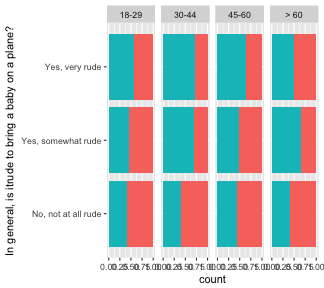
\includegraphics{Submitted_Group_Project_Storyboard_files/figure-latex/unnamed-chunk-43-1} \end{center}

\begin{itemize}
\tightlist
\item
  We can see that the average ranking of left-handed players is much
  lower than the right-handed players among 33weeks.
\item
  What about the trend of average ranking for left-handed players and
  right-handed players from 2015 to 2018?
\end{itemize}

\subsubsection{Among 2015-2018}\label{among-2015-2018}

\begin{itemize}
\tightlist
\item
  Similarly, we got the common ranking weeks data set of average ranking
  for all left-handed players and right-handed players from 2015 to 2018
\end{itemize}

\begin{verbatim}
## # A tibble: 6 x 4
##   `ranking weeks` frequency hand   year
##             <int>     <int> <chr> <dbl>
## 1              46       882 R      2015
## 2              46       132 L      2015
## 3              46       657 R      2016
## 4              46       101 L      2016
## 5              48       780 R      2017
## 6              48       122 L      2017
\end{verbatim}

And got the average ranking for left-handed players and right-handed
players from 2015 to 2017 in their ranking period.

\begin{verbatim}
## # A tibble: 90 x 4
##    month     n hand   year
##    <dbl> <dbl> <chr> <dbl>
##  1     1  743. R      2015
##  2     2  737. R      2015
##  3     3  731. R      2015
##  4     4  719. R      2015
##  5     5  713. R      2015
##  6     6  706. R      2015
##  7     7  705. R      2015
##  8     8  706. R      2015
##  9     9  706. R      2015
## 10    10  709. R      2015
## # ... with 80 more rows
\end{verbatim}

Then we plot the data by bar chart.

\begin{Shaded}
\begin{Highlighting}[]
\KeywordTok{ggplot}\NormalTok{(Sampleall,}\KeywordTok{aes}\NormalTok{(}\DataTypeTok{x=}\NormalTok{month,}\DataTypeTok{y=}\NormalTok{n,}\DataTypeTok{fill=}\NormalTok{hand)) }\OperatorTok{+}
\StringTok{ }\KeywordTok{geom_bar}\NormalTok{(}\DataTypeTok{stat=}\StringTok{"identity"}\NormalTok{, }\DataTypeTok{position=}\KeywordTok{position_dodge}\NormalTok{())}\OperatorTok{+}
\StringTok{  }\KeywordTok{facet_wrap}\NormalTok{(}\OperatorTok{~}\NormalTok{year)}\OperatorTok{+}
\StringTok{  }\KeywordTok{scale_x_continuous}\NormalTok{(}\DataTypeTok{breaks =} \KeywordTok{seq}\NormalTok{(}\DecValTok{1}\NormalTok{,}\DecValTok{12}\NormalTok{,}\DecValTok{1}\NormalTok{))}
\end{Highlighting}
\end{Shaded}

\begin{center}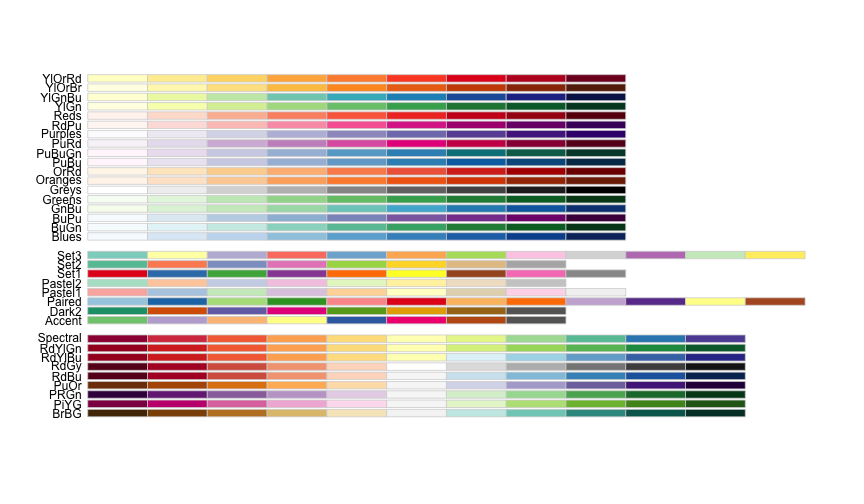
\includegraphics{Submitted_Group_Project_Storyboard_files/figure-latex/unnamed-chunk-46-1} \end{center}

\begin{itemize}
\tightlist
\item
  It can be clearly seen that right-handed players ' average ranking are
  better than left-handed players in 2015 and 2016, and left-handed
  player's average ranking are better than right-handed players in 2017
  and 2018.
\end{itemize}

\subsubsection{What we learnt}\label{what-we-learnt}

\begin{itemize}
\tightlist
\item
  Actually there is no direct relationship between the right-handed and
  left-handed.
\item
  The left-handed forehand usually likes to hit the right-handed
  backhand, which is a problem of habit.
\item
  It is considered that backhand is not good to return the ball, and
  this is exactly the forehand that left-handed people can make
  strength.
\item
  So there is a saying that left-handed people have an advantage over
  right-handed people, but it doesn't directly affect player rankings.
\end{itemize}

\subsection{Winners and Losers}\label{winners-and-losers}

\subsubsection{Tidy the data}\label{tidy-the-data}

\begin{itemize}
\tightlist
\item
  For exploring topic 4, we use a ATP data file from ``deuce'' package
  named as ``atp\_matches''. In this original data file, it has a lot of
  missing(NA) values. Furthermore, not all of the variables are what we
  want to focus on. Thus, we use the following code to tidy the original
  data file:
\end{itemize}

select(year,tourney\_name,surface,winner\_name,loser\_name)
\%\textgreater{}\% na.omit(matches)

\begin{itemize}
\tightlist
\item
  i.e.~at first, selecting the variable we want. second, exclude the na
  values.
\end{itemize}

\subsubsection{Count the no. of winnings and losings for each
players}\label{count-the-no.-of-winnings-and-losings-for-each-players}

\begin{verbatim}
## # A tibble: 12,816 x 2
##    winner_name         n
##    <chr>           <int>
##  1 Roger Federer    1218
##  2 Jimmy Connors    1197
##  3 Ivan Lendl       1065
##  4 Rafael Nadal     1007
##  5 Guillermo Vilas   932
##  6 Novak Djokovic    889
##  7 John Mcenroe      881
##  8 Andre Agassi      870
##  9 David Ferrer      855
## 10 Joao Sousa        835
## # ... with 12,806 more rows
## # A tibble: 22,710 x 2
##    loser_name                 n
##    <chr>                  <int>
##  1 Joao Sousa               695
##  2 Paolo Lorenzi            540
##  3 Feliciano Lopez          536
##  4 Ruben Ramirez Hidalgo    536
##  5 Fabrice Santoro          498
##  6 Albert Montanes          480
##  7 Andreas Seppi            474
##  8 Guillermo Garcia Lopez   474
##  9 Mikhail Youzhny          472
## 10 Teymuraz Gabashvili      470
## # ... with 22,700 more rows
\end{verbatim}

\begin{itemize}
\tightlist
\item
  Clearly, Roger Federer hits the winners most for 1218 times during
  1997-2018.
\item
  The second is Jimmy Connors who hits the winners for 1197 times from
  1970-1995.
\item
  Joao Sousa hits the losers most for 695 times from 2014 to 2018.
\end{itemize}

\subsubsection{Roger Federer's Career
growth}\label{roger-federers-career-growth}

\begin{center}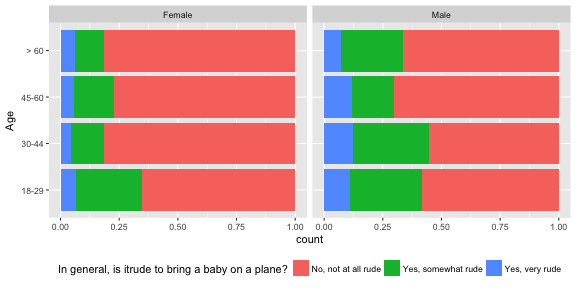
\includegraphics{Submitted_Group_Project_Storyboard_files/figure-latex/unnamed-chunk-49-1} \end{center}

\begin{center}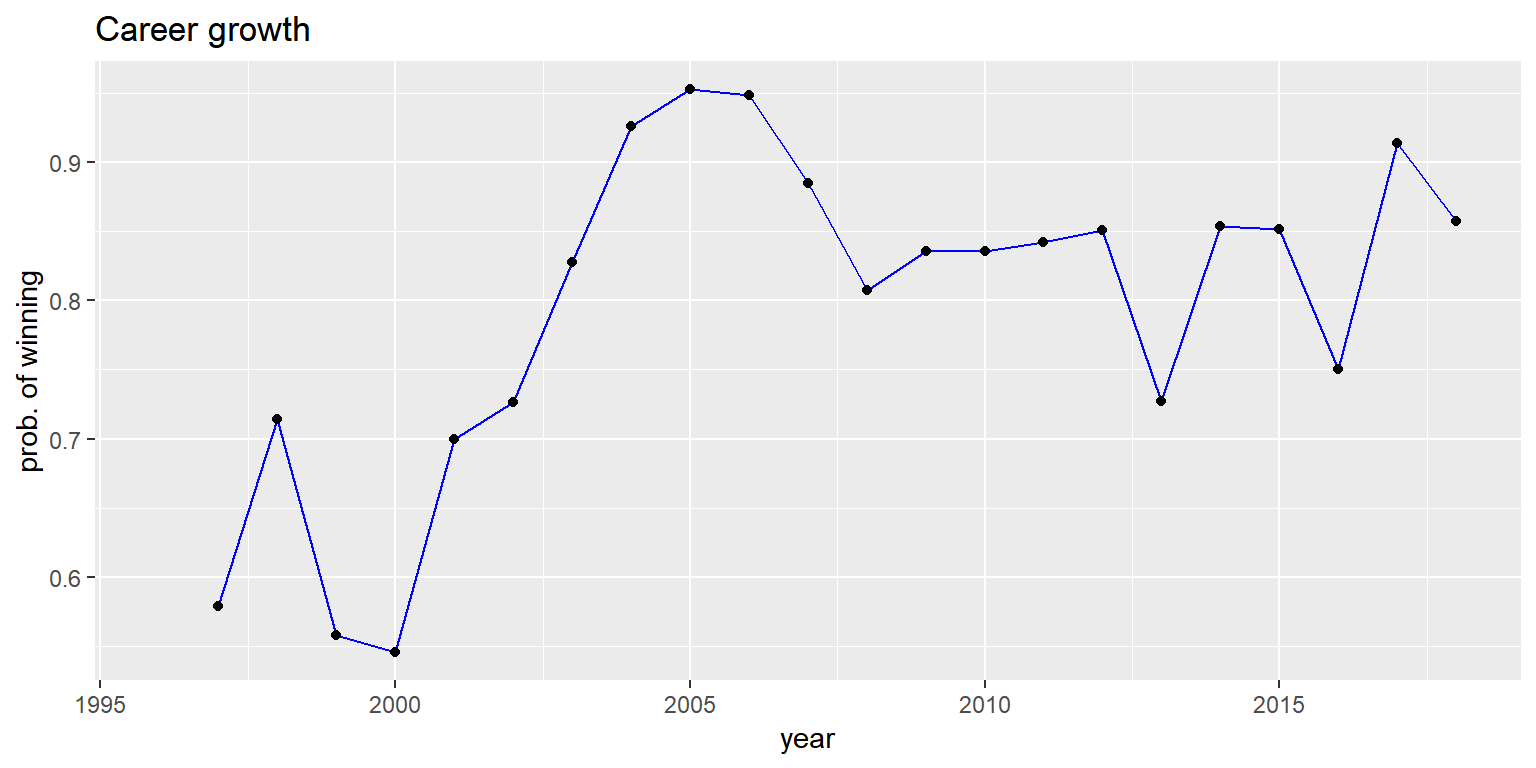
\includegraphics{Submitted_Group_Project_Storyboard_files/figure-latex/unnamed-chunk-49-2} \end{center}

\begin{itemize}
\tightlist
\item
  By looking at the above 2 graphs, Roger Federer started his career in
  1997.
\item
  Federer was ranked in the top 100 in the world in 1998.
\item
  His tennis career has grown steadily since 2000 and reached his peak
  in 2005/2006.
\item
  From 2008, his grades slipped due to Infectious
  mononucleosis(disease), and reached his trough in 2013 due to both
  illness and injury.
\item
  After 2014, it is shown a up-down volatility trend due to intermittent
  injuries.
\end{itemize}

\subsubsection{Jimmy Connors's Career
growth}\label{jimmy-connorss-career-growth}

\begin{center}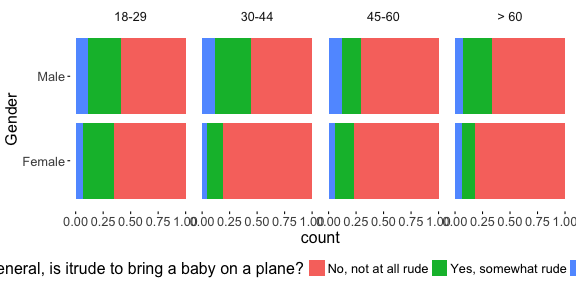
\includegraphics{Submitted_Group_Project_Storyboard_files/figure-latex/unnamed-chunk-50-1} \end{center}

\begin{center}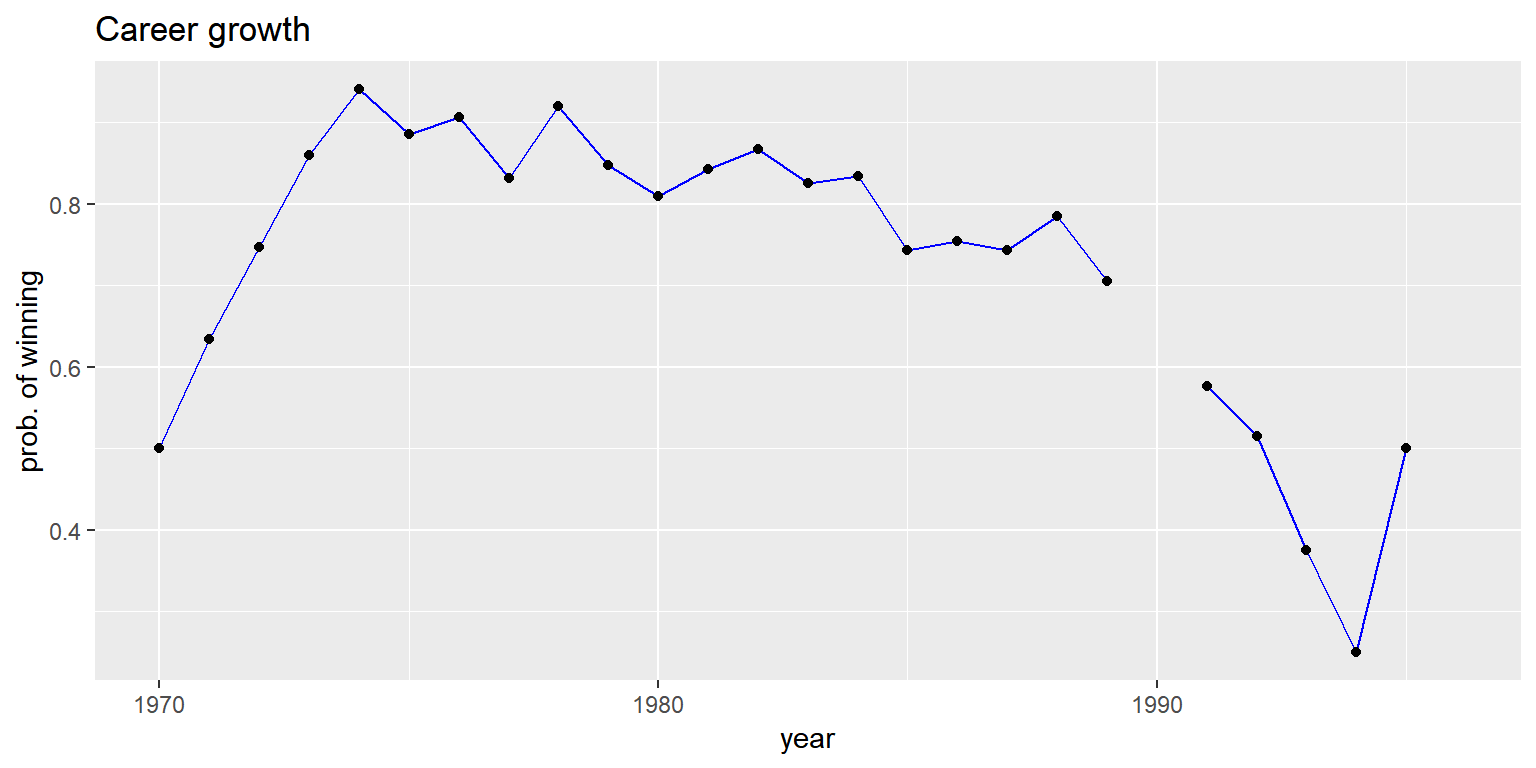
\includegraphics{Submitted_Group_Project_Storyboard_files/figure-latex/unnamed-chunk-50-2} \end{center}

\begin{itemize}
\tightlist
\item
  By looking at the above 2 graphs, Jimmy Connors started his career in
  1970.
\item
  During 1970 and 1974, his career shows significant growth.
\item
  After that, it is shown a gradual decline and he retired in 1995
  finally.
\end{itemize}

\subsubsection{Joao Sousa's Career
growth}\label{joao-sousas-career-growth}

\begin{center}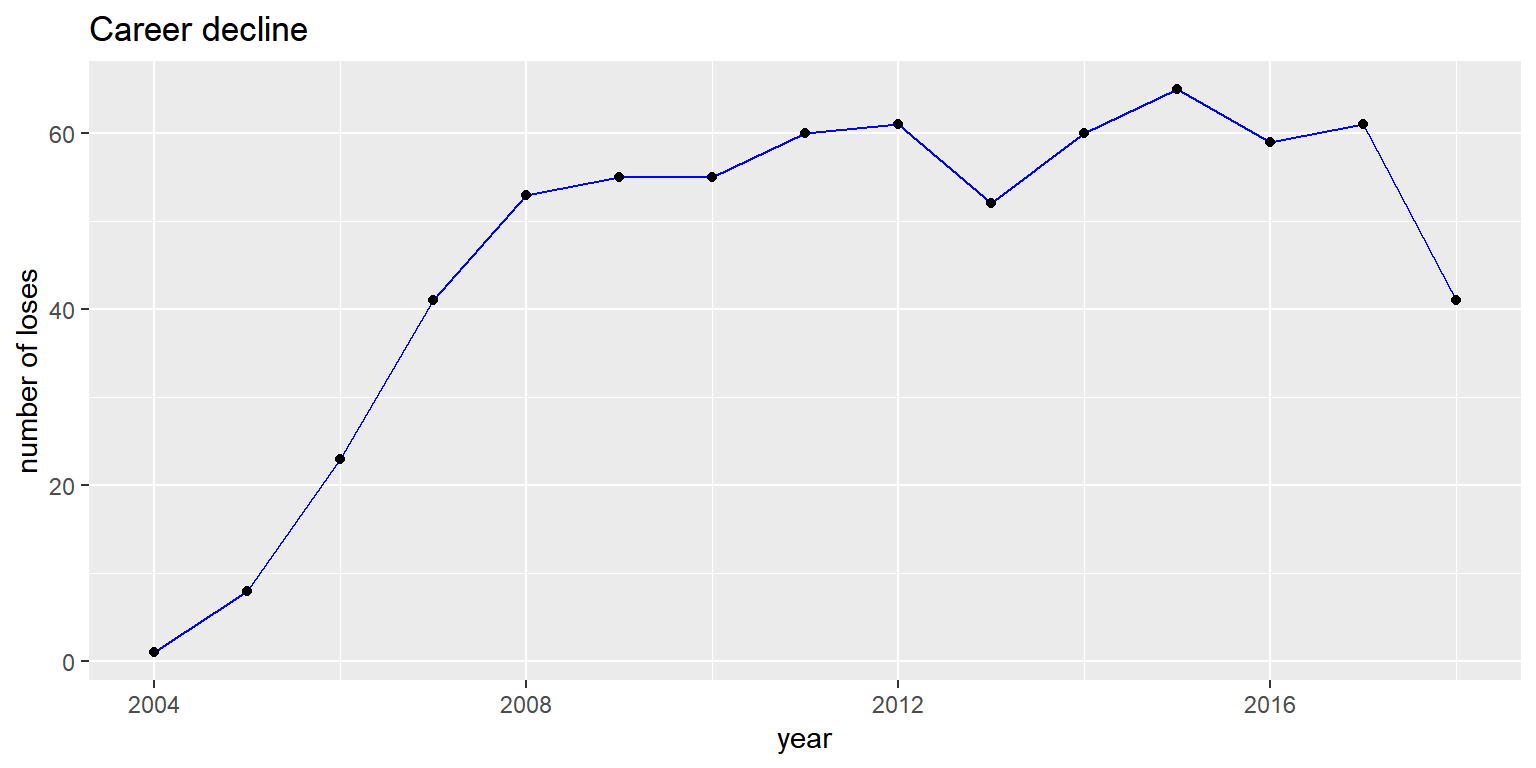
\includegraphics{Submitted_Group_Project_Storyboard_files/figure-latex/unnamed-chunk-51-1} \end{center}

\begin{center}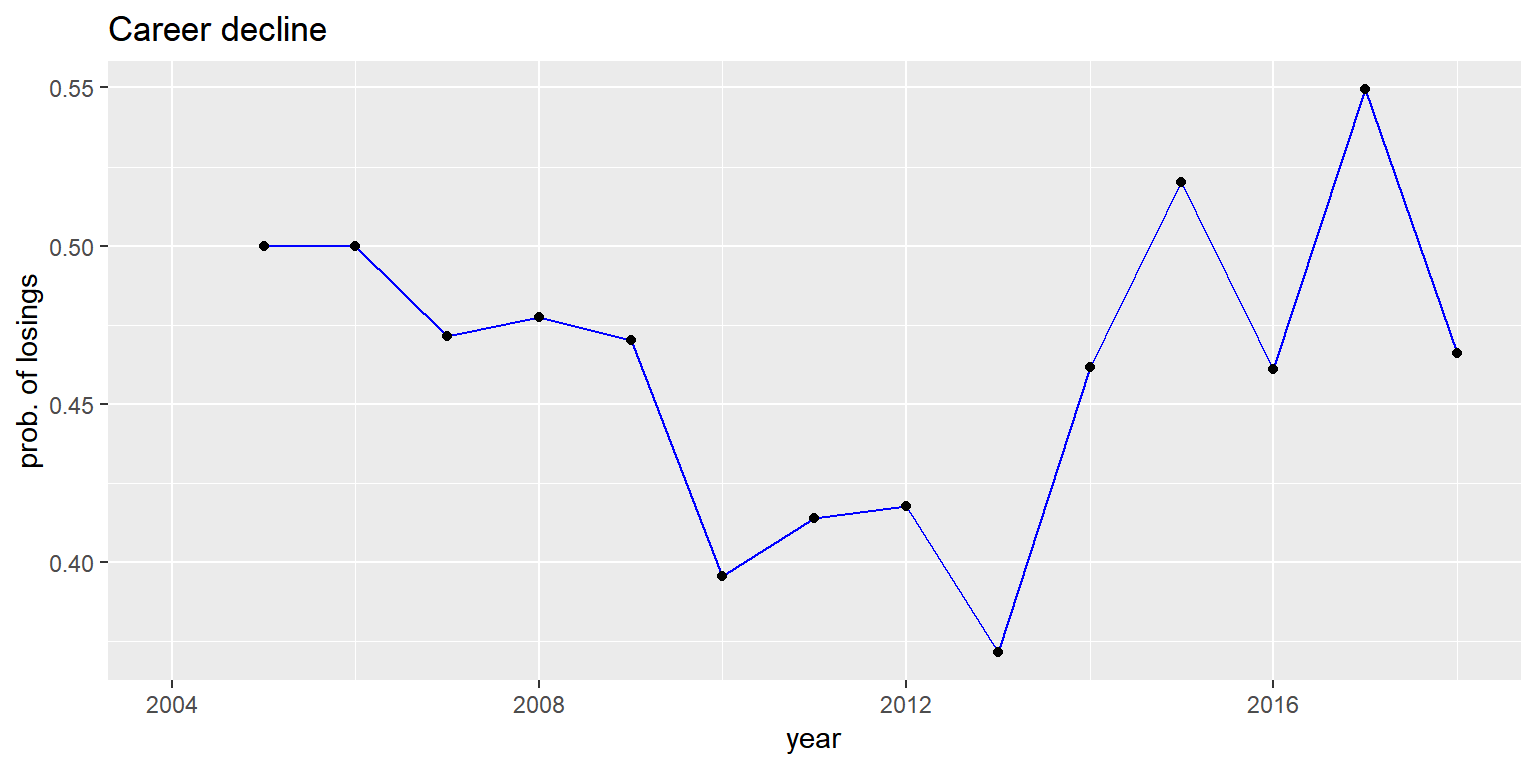
\includegraphics{Submitted_Group_Project_Storyboard_files/figure-latex/unnamed-chunk-51-2} \end{center}

\begin{itemize}
\tightlist
\item
  By looking at the overall trend from 2004 to 2018, there's no doubt
  that Joao Sousa's professional career is a decline since the
  probability of losings and the times of being losers increase year by
  year.
\end{itemize}

\subsection{THANKS FOR LISTENING! :)}\label{thanks-for-listening}


\end{document}
